%------------------------------------------------------------
% thesis - Andy Taylor 
%------------------------------------------------------------
\documentclass[11pt,a4paper,titlepage,twoside,openrigh]{book}
\usepackage{style/uomthesis}  % Unimelb thesis template
%---------------------------
% formats and definitions
%---------------------------
%\newcommand{\markblankpages}{}     % option:"This page intentionally left blank."
%\newcommand{\archivalpapernote}{}  % option: copy submitted to the library
% add DRAFT water mark
\usepackage{draftwatermark}
\SetWatermarkText{DRAFT} 
\SetWatermarkLightness{0.98}
\SetWatermarkAngle{45}
\SetWatermarkScale{1.2}
                % draft watermark
%-----------------------------------
% Packages
%-----------------------------------
\usepackage{setspace}
\onehalfspacing
\usepackage{natbib}
\usepackage{enumerate}
\usepackage{subcaption}
\usepackage{float}
\usepackage{paralist}
\usepackage{amssymb}
\usepackage{amsmath}
\usepackage{amsthm}
\usepackage[mathscr]{eucal}
\usepackage{graphicx}
\usepackage[hidelinks]{hyperref}
%-----------------------------------
% figure size defaults
%-----------------------------------
\newlength{\myfigwidth}
\setlength{\myfigwidth}{400pt}
%-----------------------------------
% References
%-----------------------------------
\bibliographystyle{bib/ametsoc2014}
%------------------------------------------------------------------------
% colours & symbols
%------------------------------------------------------------------------
\usepackage[framemethod=tikz]{mdframed}
\usepackage{color}
\definecolor{mygrey}{rgb}{0.9,0.9,0.9}
\definecolor{mygreen}{rgb}{0,.4,0}
\usepackage{listings}
\lstset{
language=bash,                   % Code langugage
backgroundcolor=\color{mygrey},  % choose the background color; you must add \usepackage{color} or \usepackage{xcolor}
basicstyle=\ttfamily,            % Code font, Examples: \footnotesize, \ttfamily
commentstyle=\color{mygreen},    % comment style
breaklines=true,
}
% bullet symbol
\renewcommand{\labelitemi}{{\tiny$\blacksquare$}}
% highlights
\newcommand{\BoxBegin}{\begin{mdframed}[hidealllines=true,backgroundcolor=yellow!30]}
\newcommand{\BoxEnd}{\end{mdframed}}

% matrices etc
\newcommand{\M}[1]{\mathsf{#1}}
\newcommand{\V}[1]{\mathbf{#1}}

%-----------------------------------
% config
%-----------------------------------
% no indents
\setlength\parindent{0pt}
% Allow equations to break over pages...
\interdisplaylinepenalty=2500
% Command to stop equation breaks
% Note: enclose this in braces when used...
\newcommand{\donotsplitoverpages}{\interdisplaylinepenalty=10000}               

%\newcommand{\figureInit}{\begin{figure}[h]\centering}
%------------------------------------------------------------------------ 
% shortcut text
%------------------------------------------------------------------------ 
\newcommand{\TITLE}{`TITLE'}
\newcommand{\ALTTITLE}{`ALT TITLE'}
\newcommand{\BOM}{Australian Bureau of Meteorology}
\newcommand{\LTE}{\textbf{\texttt{LTE}}}
\newcommand{\ATGF}{\textbf{\texttt{ATGF}}}
\newcommand{\ATGP}{\textbf{\texttt{ATGP}}}
\newcommand{\SSH}{\textbf{\texttt{ssh}}}
\newcommand{\BL}{\textbf{\texttt{Bluelink-OceanMAPS}}}
\newcommand{\MOM}{\textbf{\texttt{MOM}}}
\newcommand{\ROMS}{\textbf{\texttt{ROMS}}}
\newcommand{\GODAE}{\textbf{\texttt{GODAE}}}
\newcommand{\OGCM}{\textbf{\texttt{{OGCM}}}}       %{\textbf{\texttt{OGCM}}}
\newcommand{\OFAM}{\textbf{\texttt{{OFAM}}}}
\newcommand{\OFAMHR}{\textbf{\texttt{{OFAMHR}}}}
\newcommand{\NWP}{\textbf{\texttt{NWP}}}
\newcommand{\OTIS}{\textbf{\texttt{OTIS}}}
\newcommand{\GOOS}{\textbf{\texttt{GOOS}}}
\newcommand{\obc}{\textbf{\texttt{obc}}}
\newcommand{\ANTT}{\textbf{\texttt{ANTT}}}
\newcommand{\CTE}{\textbf{\texttt{CTE}}}
\newcommand{\SAL}{\textbf{\texttt{SAL}}}
\newcommand{\AG}{\textbf{\texttt{ACCESS-G}}}
\newcommand{\AR}{\textbf{\texttt{ACCESS-R}}}
\newcommand{\ER}{\textbf{\texttt{eReefs}}}
            
%---------------------------
% metadata
%---------------------------
\title{On the application of conventional tidal concepts within operational sea level forecasting}
\author{Andy Taylor}
\orcid{0000-0003-1258-5002}
\submissionmonth{April}
\submissionyear{2021}
\department{School of Earth Sciences}
\university{\textsc The University of Melbourne}
%----------------------------------------
\begin{document}
    %---------------------------
    % front 
    %---------------------------
	\begin{frontmatter}
		\frontmatterheadings    % collect information for title page        
		\maketitle              % title         
		\makedeclaration        % author declaration
		
\begin{abstract}
This is the abstract
\end{abstract}
\clearpage

		
% Optional preface to the dissertation
\begin{preface}

This thesis with publication is built around the following peer-reviewed publications:

\vspace{5mm}
\hangindent=3em
\hangafter=1
Taylor, A. J. and Brassington, G. Sea Level Forecasts Aggregated from Established Operational Systems. Journal of Marine Science and Engineering 5, 33 (2017).

%\citep{Taylor:2017coa}


\vspace{5mm}
\hangindent=3em
\hangafter=1
Taylor, A. J. and Brassington, G. B. Sea Level Anomaly Forecasts on a Coastal Waveguide. Weather and Forecasting 35, 757–770 (2020).
%\citep{Taylor:2020}

\vspace{5mm}
\hangindent=3em
\hangafter=1
Extension material from the later presented at:
\vspace{5mm}
\hangindent=3em
\hangafter=1

Taylor, A., Greenslade, D., Zhou, X., and Brassington, G. (2020). National NonTidal Sea Level Forecasts on a Coastal Waveguide. Coastal Engineering Proceedings, (36v), currents.26. https://doi.org/10.9753/icce.v36v.currents.26
%\cite{10.9753/icce.v36v.currents.26}

\vspace{5mm}
\hangindent=3em
\hangafter=1
The material comprising chapter \ref{chp:tideFlavours} is in preparation for stand-alone publication.

\vspace{5mm}
\noindent  All funding and in-kind support for this research provided by the Australian Bureau of Meteorology. 

\end{preface}


		
\begin{acknowledgements}

% stop indents
{\parindent0pt

First and foremost I acknowledge the traditional ownership of the lands and seas that host Australia. These coasts have been known for so long.
\newline{}

Thanks to the ever-fantastic Kulja and our wanderings over mudflats and mangroves that first put the tides under my feet.   
    %Wetland people ..Pelican
    
%\newline{}    
    
Big thinks to Gary Brassington at the Bureau of Meteorology for making this whole effort possible.

%\newline{}

Tides  unit - James, Bill and Mike
Forecasters - James Taylor, Ben Hague and more
Phil Shinkfield , Jane Warne and more
Diana
    
The wider Bluelink community
David Griffin, Paul Sandery    
    
Unimelb
Kevin Walsh

OS early input 
Mike Foreman
Ed Zaron
%Lana and Gary E

%%%%%%%%%%%%%%%%%%%%%%%%%%%%%%%%%%%%%%%%%%
%\newline{}

Observational data shared with the Bureau from external agencies was important for this study, in particular from:
\begin{itemize}
    \item Manly Hydraulics Laboratory \url{http://mhl.nsw.gov.au/}
    \item Queensland Government Department of Environment, Land and Water \url{https://www.qld.gov.au/environment/coasts-waterways/beach/storm-sites]}
\end{itemize}


% template from git bloke	
And thanks for the LaTeX template \url{http://jpap.org/projects.html} by John Papandriopoulos.

}   % end no indent
\end{acknowledgements}

		{
			\singlespacing
			\tableofcontents
			\listoffigures
			%\listoftables   % not for less than 10 tables
		   \clearpage
		}
   \end{frontmatter}
    %----------------------------------------------
	% main
    %----------------------------------------------
	\begin{mainmatter}
		\mainmatterheadings
		\chapter{Review}  
\label{S:REVIEW} 

%--------------------------------------------------
\section{Sea level in context}

Sea level plays a unique role in physical oceanography. A role at least partly be attributed to it's \emph{observability}\citep{Wilson:2010hy}.


The present study will be limited to forecasts of sea level over time scales of hours to days; variations that basically constitute `the tides' as far as the general public is concerned.

\begin{figure}[h]\centering
  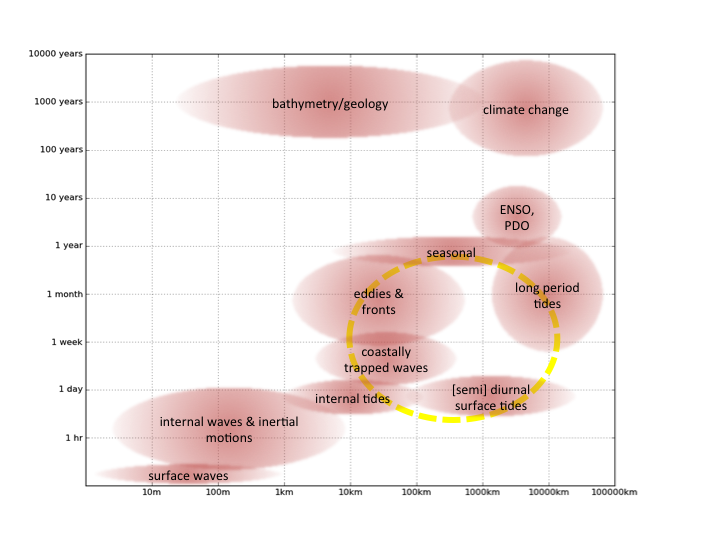
\includegraphics[width=130mm]{figures/diagrams/ocean_scales.png}
  \caption{Schematic indication of time/length scales of ocean processes.  The approximate scale limits for this research are highlighted. (Following \citet{Chelton:2001ws} )}
  \label{fig:SCALES}
\end{figure}

\begin{figure}[h]\centering
  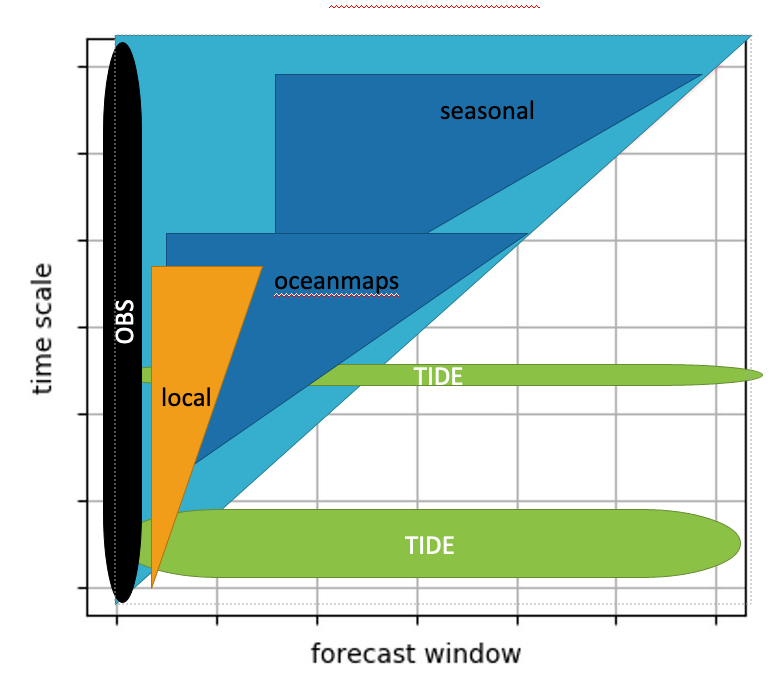
\includegraphics[width=80mm]{figures/images/sealevel_cartoon.png}
  \caption{Simplified illustration of the relative nature of sea level and different observing platforms.}
  \label{fig:SEALEVEL}
\end{figure}


\begin{figure}[h]\centering
	\subfloat[Darwin in Northern Australia - large diurnal tide.]{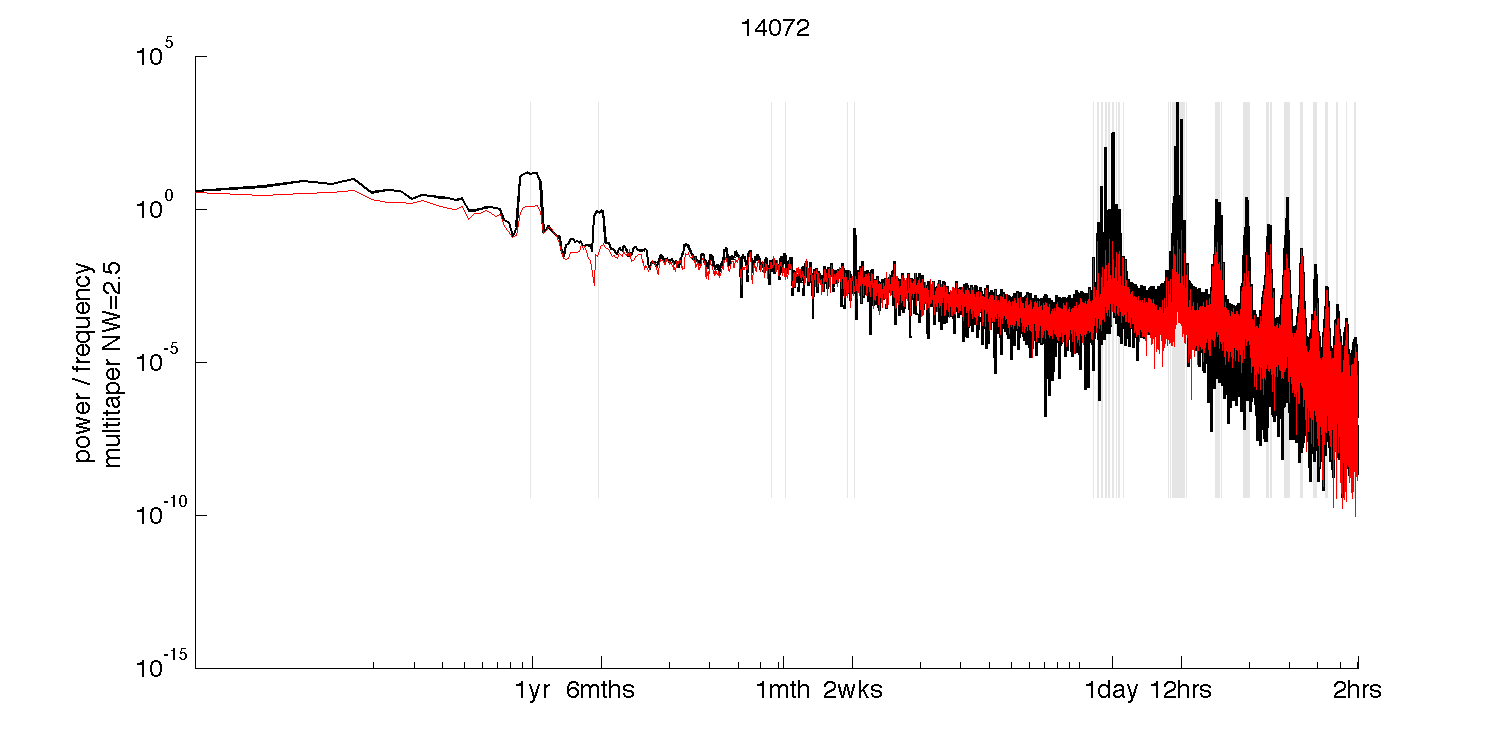
\includegraphics[width=130mm]{figures/images/plot_14072.png}} \\
	\subfloat[Esperence in Southern Australia - powerful synoptic signal.]{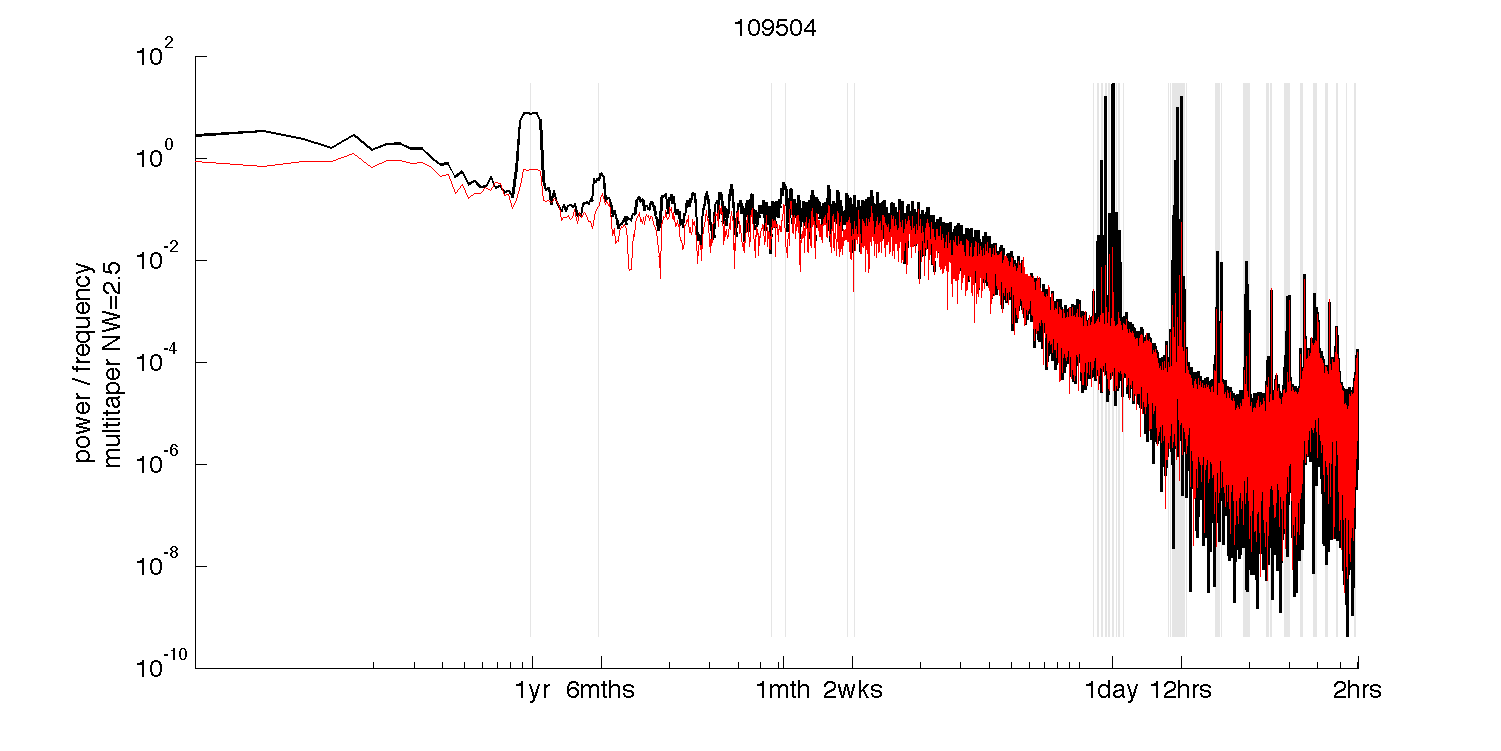
\includegraphics[width=130mm]{figures/images/plot_109504.png}}
	\caption{Spectral estimates from two coastal tide gauges. Hourly data, black = observations, red = tidal residual. An example of a `mixed spectra' \citep{Percival:1998tw}, in the sense of that discrete spectral lines appear embedded in a background continuum of coloured noise.  The overall `redness' of the spectra and the prominence of spikes at tidal frequencies is highlighted }
    \label{fig:SPECTRA_EG}
\end{figure}


%--------------------------------------------------
\subsection{TBC - towards more obs and SWOT}

More real time obs.

Remote obs - SWOT - need for corrections and ground truthing....


%--------------------------------------------------
\subsection{Operational forecast setting}
\label{S:operational_setting}

Operational considerations are relevant to this review, which does not launch neatly from a single `conversation' \citep{Booth:2009vy} in the scientific literature.\\
Unfortunately operational documentation often falls far behind aspirations.
Tidal observation manuals exist eg \citep{IOC:2005tj}, \citep{Level:2011wu}, \citep{Parker:2007wq}.  However, analysis methods and design justifications are less formally documented - if at all.  The IOC understates this situation simply: `many organizations have developed their own method of tidal analysis'\citep{IOC:2005tj}\\

User expectations of sea level forecasts have largely been defined by harmonic tidal prediction practice. 
Conversely operational practice have influenced oceanography more broadly. Doodson's \citep{Doodson:1928wf} tidal procedures reflect the practical limits imposed by human computers and paper records, but have ongoing influence. \\


%--------------------------------------------------
\subsection{Future directions for forecast development}

BoM research strategy.


More general:

\begin{itemize}
  \item Towards 'concrete' , increasingly realistic and inclusive primitive equation forward models.
Peterson M1 ]\citep{Petersen:2012tr}
 \item Towards data-driven, service target - idealised, simple and robust 
\end{itemize}

%-------------------------------------------------- 
\subsection{Intersection of prediction perspectives}
\label{S:two_perspectives}

Tidal harmonic methods have for many decades provided the only routine source of sea level forecast - and with great success.  
In contrast, time stepping primitive equation dynamic models and data assimilation are relatively new arrivals to operational centres.  
These represent two qualitatively different perspectives on sea level prediction.\\


Over the past decade, the operational evolution of \OGCM-based prediction has increasingly brought the two approaches into something akin to Gallison's `trading zone' \citep{Galison:1996uc}.
Developments promise only to increase the amount of overlap into the previously independent practices of harmonic analysis, eg \cite{Arbic:2010us}.\\
Here Munk and Cartwright's aphorism from the 1960's regarding tidal analysis is illustrative:
\begin{quote}
  \dots predicting and learning are in a sense orthogonal, and the most interesting effects are those that cause the most trouble with a forecasting: the continuum, the nongravitational tides, and the non-linear interactions.\citep{Munk:1966ts} 
\end{quote}
Forecasts from \BL{} and other similar systems now represent sea level attributable to exactly these troublesome areas; or at least some physical subset therein.
Jayne's reference to the ``vexing problems'' \citep[pp812]{Jayne:2001tr} arising from applying frequency-domain theory in time-domain numerical tide modelling is illustrative.

\begin{figure}[h]\centering
  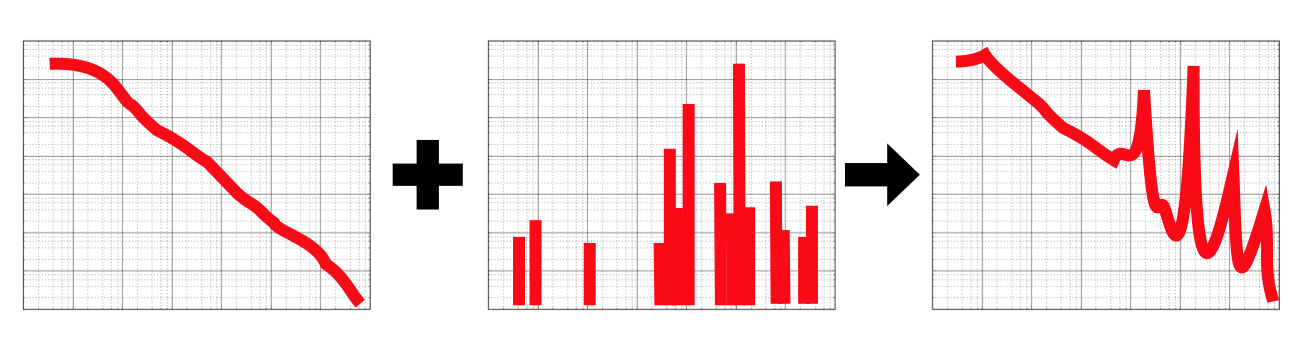
\includegraphics[width=120mm]{figures/diagrams/spectra_cartoon_1.png}
  \caption{Conventional decomposition concept: mixed sea level spectra comprising discrete tidal `lines' and red turbulent continuum.  Implementation of this concept has ramifications for sea level forecasting.}
  \label{fig:SPECTRA_CARTOON}
\end{figure}

Viewing sea level as a stationary set of harmonics is at face value quite at odds with a view of the ocean as a turbulent fluid.   In that sense, Gallison's portrayal of physics as `neither unified nor splintered into isolated fragments' \citep[pp 782]{Galison:1987wh} is apt.  Thus also is Peterson's assertion of `\dots{} the fundamental plurality of \dots{} scientific practice' \cite{Petersen:2012tr}. 

\section{Operational oceanography}
\label{S:operational_oceanography}

Mesoscale ocean prediction moved into operations across the early 2000s in a manner that lagged and imitated the path of NWP \citep{Harper:2008ub}. Operational oceanography is `big science' \citep{Petersen:2012tr} in the sense that it fundamentally relies on the coordination of large organisations, global networks and capital. \\
Starting in 1997, the international collaboration of the Global Ocean Data Assimilation Experiment \GODAE{} serves as a historical reference point:

\begin{quote}
  The central idea of \GODAE{} - to demonstrate the feasibility and utility of real-time, global ocean forecasting - was based on the experiences of the meteorological community in \dots{} FGGE. \citep{Bell:2009uv}
\end{quote}


%-----------------%
\subsection{Ocean General Circulation Models}

Since \GODAE{}, Ocean General Circulation Models (\OGCM{}s) are a key component in operational oceanography.\\

An \OGCM{} simulates the physical ocean state via time-stepping a mixed boundary-/initial-condition problem.\citep{Griffies:2004vs}.\\
A distinction between \emph{resolved} and \emph{unresolved} scales is paramount.  `Sensitive dependence on initial conditions in this turbulent flow \dots{} severely limits predictive capabilities [and] motivates a formulation of averaged or mean field fluid equations' \citep[Sec 2.5]{Griffies:2004vs}.\\


Information cascades between turbulent scales places importance on sub-grid scale (SGS) parameterisations; and raises broad questions of representiveness.\\
Griffies perceives an \OGCM{} as representing the averaged motion of an infinite ensemble of hypothetical oceans; the imagined spread being proportional to the scales of SGS parameterisation.
Alternatively, Stevens casts \OGCM{}s into the class of geophysical `pseudofluid' simulations \citep{Stevens:2001kb}. Of which he notes comparisons with observational data are prone to interpretational nuance and are ``too often ad hoc, uncritical, and/or irrelevant''\citep[pp 286]{Stevens:2001kb}. \\

\begin{figure}[h]\centering
  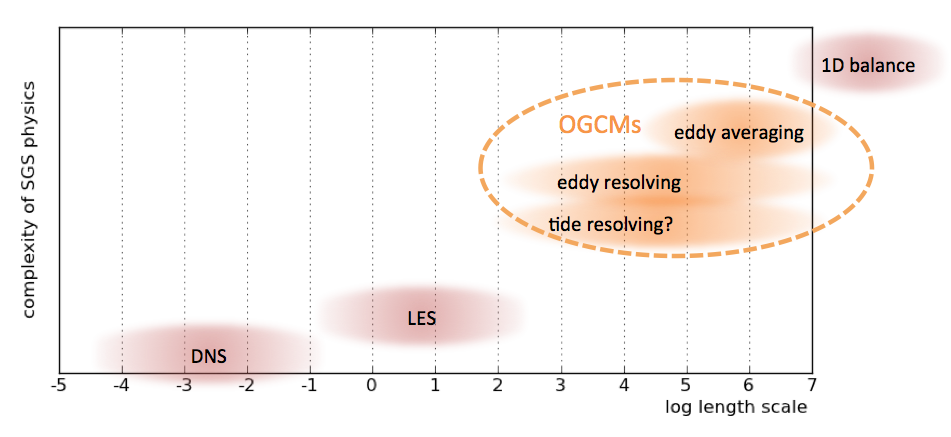
\includegraphics[width=120mm]{figures/diagrams/model_types_schematic.png}
  \caption{Schematic illustration of place of \OGCM{}s in terms of SGS parameterisation of the broad scale range of a turbulent ocean.  For reference, methods from turbulence studies are included: Direct Numerical Simulation and Large Eddy Simulation. Following \citep[fig 5.2]{Petersen:2012tr} and \citep{Stevens:2001kb}.  Inclusion of explicit tides is tentatively placed as a reduction of parameterisation without increased spatial scale resolution.}
  \label{fig:models}
\end{figure}

Common to `big science' simulation practice \citep{Petersen:2012tr} an \OGCM{} embodies a large amount of collective and accumulated programming effort in many lines of computer code; too much for any one person to understand in detail. \\



%-----------------%
\subsection{Ocean observations and data assimilation}
Data assimilation is the framework for combining information from ocean observations and the chaotic dynamics embodied by an \OGCM{}; usefully viewed from a Bayesian perspective\citep{Zaron:2011ft}.\\
Despite the growth of \GOOS{} \citep{Komen:1999ch}, the ocean is fundamentally under-observed for the purposes of physical state estimation.\\


Satellite-based ocean altimetry provides a data stream of special significance to contemporary ocean forecasting \citep{Fu:2001ub}. \\
Derivation of sea level quantities from satellite mounted radar instruments is particularly challenging in shallow water and near coastal boundaries \citep{Woodworth:2011bf}. 
Altimetry has directly enabled contrasting scientific developments in global tides (eg.\citet{Egbert:1996vr},  \citet{Lefevre:2011dg}) and mesoscale ocean variability (eg.  \citet{Wunsch:1998bq}, \citet{Chelton:vi}).

 
% segue into OGCM
%--------------------------------------------------
%--------------------------------------------------
\subsection{Treatment of tides in \OGCM{}s}
\label{S:tides_ogcm}
To date \OGCM{}s in the \GODAE{} heritage have focused on nominally \emph{nontidal} ocean dynamics, with de-tided sea level observations playing a unique role.\\


From that background, recent publications indicate a motivation towards more dynamic representation of the effects of ocean tides.   This is indicative of pervasive goal across numerical simulation practice to increase model concreteness by reducing the role of parameterisations \cite[section 5.3]{Petersen:2012tr}; a reduction of system aggregation \citep{Stevens:2001kb}.\\
Similarly, Griffies describes the ``general trend in ocean climate modelling towards reducing many of the common approximations'' \citep[pp20] {Griffies:2004vs}.
It could be said that the modelling community perceives parameterisations as a compromise that should ideally be replaced with explicit physics when computing power allows.  In spite of this, operational justification is a separate matter.


%-----------------%
\subsection{Nominally non-tidal \OGCM{}s}
\label{S:nontidal}

\BL{} is a nontidal system in that no gravitational body forcing associated with the \ATGP{} is applied.   Subsequently, assimilated observations of sea level are corrected (filtered) using pre-computed global tide models.  The state variable quantifying surface elevation carried by the model is termed sea level anomaly (SLA) which in itself is a rather abstract quantity. Using Stevens' nomenclature, \BL{} simulates an aggregated pseudofluid system with a qualified relationship to the actual ocean.


% split 
Timescales for depth-integrated barotropic and depth-dependant baroclinic ocean state are quite distinct and the design of \OGCM{}s have been influenced by this distinction. \\
%rigid ild
One approach has been to make the so-called `rigid-lid' approximation \cite[pp128]{gill1982atmosphere}. 
The rigid-lid by definition cannot represent explicit barotropic tides, and has other ramifications for ocean forecasting \cite[pp19]{Griffies:2004vs}.\\


% split explicit
A compromise strategy employed in \MOM{} (and other \OGCM{}s) is the so-called `split-explicit' scheme.    
In essence, cheap shallow-water barotropic dynamics are timestepped many times for each relatively expensive update of the full depth-dependant ocean state.  \\
Thus \MOM{} at face value is capable of representing barotropic surface tides.   However, there are several high level arguments against doing so.\\
One reason is the aims to which the model is being employed.  Much of the development of \OGCM{}s has been focused at climate times-scales, tipping the balance of away from the accuracy of high frequency sea level signals.   
Furthermore, in comparison to highly tuned tidal altases, simple and general barotropic can't be expected to achieve similar skill.\\

Filtered altimetry observations provide great value in observing and forecasting mesoscale eddies.
Treating tides as noise is reasonable insofar as the effects on the mesoscale structure are small relative to other source of error.\\

Decomposition of the dynamics into tractable categories for simulation is not aggregation per se, but it certainly does have implications for the role of parameterisations.  \\

From the perspective of \emph{users} of ocean forecasts there is basically no inherent value in decomposition.   
 
%-----------------%
\subsection{Motivation to explicitly resolve tides}

As processing capacity increases, compromises imposed by past computing limitations are re-contextualised.   Inclusion of explicit tides within \OGCM{}s is increasingly affordable from a computational perspective.

With developments to date, exploration of this possibility has been directed primarily at the influence of barotropic tides on the baroclinic structure of the ocean state.   \\


% tides <-> baroclinic
Barotropic tides do interact with the baroclinic structure of the ocean, which conversely impacts the behaviour of barotropic waves and the \emph{non-constant} \citep{Ray:2010jm} nature of tidal constants.\\

Beyond the general simulation goals of model concreteness, it is the possible significance of barotropic/baroclinic interactions for global circulation that provides the primary motivation for considering explicit resolution of tides within \OGCM{}s.   



%-----------------%
\subsubsection{Temporal formulation of tidal forcing}
\label{S:numerical_impl}

The astronomical tidal forcing can be conceptualised as a relatively smooth global surface field that varies in time. 
Perhaps the most significant numerical implementation consideration is how this time variation is formulated.\\


At face value, the \underline{direct formulation} provides the most unmediated and accurate representation of $\eta_{eq}$. Given spherical harmonics $(n,m) \in (2,0) , (2,1) , (2,2)$, the full global tidal forcing can be pre-computed $c_{nm}(t)$ as 6 real valued time series and simple trigonometric functions of location.\\
This approach has the advantage of accurately representing the \ATGP{} and facilitates incorporation of best-practice pre-computed SAL corrections \citep{Egbert:2002ug}. \\
Furthermore, this approach could offer consistent numerical formulation with other barotropic forcing fields.\\


On the other hand, some programatic inconveniences and risks are introduced. 
The input time series must be extracted from the ephemerides at timings to suit each particular simulation.  Furthermore, the extraction process is relatively opaque and would require cross-checks to mitigate the risk of non-fatal errors arising for file dependancies (e.g. incorrect dates).\\
Direct forcing is apparently not as common in the ocean literature as in gravity related studies.   
One instance of forcing a global hydrodynamic model directly is described by Weis and Sunderman \citep{Weis:2008ex} - notably in an non-operational setting.\\\



In contrast, a \underline{harmonic formulation} of $c_{nm}(t)$ for the same range of spatial harmonics requires the specification of many constants for each \emph{temporal} harmonic to be included.  
Hundreds of harmonic components \citep[pp3]{Desai:2006wo} would be required to match the spectral content of an equivilant direct formulation.\\

In practice only a small number (often 8) of the most powerful spectral clusters are specified as `primary constituents'.  
Truncation is based on the relative power of tidal lines within the harmonic development and subsequently requires nodal adjustments (as per Equation \ref{E:Axb}).

Programatically the harmonic approach facilities some attractive simplifications.  
After the specification of a small number of constants, the temporal variation can be cheaply calculated within the ocean model via only a few lines of code.   
For relatively short simulations ($\ll$ 1 year), the nodal corrections are reasonably treated as fixed.   This situation is amenable to de-bugging and has no external dependancies.\\
It is also a relevant consideration that assessment of tidal output is conventionally based on harmonic fits to these same primary constituents.\\

Arbic et al \citep{Arbic:2010us}, apply body forcing using the temporal harmonic representation.  In what appears to be common approach the authors describe developing their implementation via a progressive addition of temporal harmonics: no tides, M2-only, 8 primary constituents.  Treating M2 separately facilitates interpretation and comparison to other literature; including theoretical developments of single frequencies and tidal atlases.



%MOM
The public distribution of \MOM{} includes a very simple module for representing tidal body forcing in a manner suitable for climate simulations\cite[pp263] {Griffies:2008vh}.\\
The eight most powerful constituents (frequency clusters) from $\eta_{eq}$, due to only spherical harmonics $(n,m) = (2,1) , (2,2)$, are written with fixed harmonic amplitude.  SAL is simply parameterised with the scalar approximation. \\
Astronomical phase information is neglected altogether.
Schiller and Feidler \citep{Schiller:2007gk} worked around this gap with addition of a hard-coded astronomical argument offset valid for a particular epoch.\\
Tidal body forcing is written as a depth-independent horizontal term in the momentum equation evolved at the barotropic timestep.
This cheap barotropic code reflects the climate-simulation background of \MOM{}.  
By default, arbitrary forcing terms such as surface fluxes are held constant over iterations of the inner barotropic loop.  
Whilst this is a reasonable optimisation given relatively slow forcing timescales, it is not valid for $\eta_{eq}$ which varies powerfully and quickly.
By employing the temporal harmonic approach to representing the tidal force, $\eta_{eq}$ can be updated algebraically at the barotropic timestep, without requiring relatively expensive file input/output.\\




\subsubsection{Other Aspects of Formulation}
Beyond the basic \ATGP{}, there may be some prospect for translating forcing corrections from \emph{tidal} data assimilation models to an \OGCM{}. \\
The \underline{Generalised Inverse} (GI) \cite[pp345] {Zaron:2011ft} approach employed by \OTIS{} \cite{Egbert:2002ug}, draws an objective trade-off between observational and dynamic uncertainties; the ``inevitably approximate nature of the discretised dynamical constraints''\cite[pp155]{Egbert:1996vr}.  The inversion process involves determining adjusted forcing to achieve the optimal trade off.\\
Thus it is speculated that complementary use of \OTIS{} may be exploited to improve the representation of a stationary tidal signal in the time-stepping \OGCM{}.  \\


%OBC
Application of tidal forcing to a \emph{regional} prediction system raises the topic of open boundary conditions (\obc{}).  \obc{}s are of fundamental importance for limited area ocean models but review is considered beyond the scope of this document at present.\\


%-----------------%
\subsubsection{Vertical Mixing}

% climate mixing
An emphasis on improving the representation of \emph{baroclinic} circulation is apparent in \OGCM{} simulations implementing explicit tides.\\
Simmons et al \citep{Simmons:2004fi} are motivated to increase the concreteness of parameterisations with regard to the conversion of barotropic tidal energy.  Surface elevations were not the target of these simulations. \\


% schiller MOM
At timescales closer to those of operational forecasts, Schiller et al have also employed explicit tides within free-surface configurations of \MOM{}.  
Better representation of baroclinic mixing is again a primary motivation. 
Specifically, improved understanding of water mass structures \cite{Schiller:2004fv} and upper ocean circulation \cite{Schiller:2007gk} were cited as justifications for the implemention.  
Whilst the resolution of these configurations did not aim to resolve internal tide processes, explicit barotropic tidal currents enabled vertical mixing parameterisations to reflect spatially and temporally varying tidal effects.\\
In addition to the focus on mixing, surface level skill was evaluated against a coastal tide gauge and shown to offer some promise as a prognostic output \citep[Fig 2]{Schiller:2007gk} - apparently despite expectations.   
The issue of top-layer thickness limitations on surface elevation magnitudes highlighted by the authors does not directly apply to the contemporary \BL{} configuration of \MOM{}, which employs the $z^*$ coordinate \citep{Brassington:2012wm}.\\


%-----------------%
\subsubsection{Conversion Parameterisation}

% wave drag
Bringing astronomical forcing effects from `parameterised' to 'resolved' is a significant change with ramifications for parameterisation settings generally. \OGCM{}s parameterisation typically do not scale well.\\



Arbic et al \cite{Arbic:2004wz} discuss the `inordinately large' bottom drag values required by hydrodynamic tidal models and argue for the value of additional topography-based parameterisations.   
For example, the wave drag scheme described by Jayne \cite{Jayne:2001tr} is designed to spatially align barotropic dissipation over features such as mid-ocean ridges that are known to be source of internal tide generation.  Whilst a spatial concentration over internal tide generation locations is attractive - the relationship to vertical mixing may be misaligned to the extent that the energy cascade is non-local.  Internal wave propagation has a frequency/latitude dependance, with a qualitative transition from propagating to trapped occurring poleward of critical latitudes.  Furthermore `` the extent to which internal tides produce turbulence as they propagate away from their generation sites is not clear'' \citep[pp812]{Jayne:2001tr}.\\



It is notable that a related scheme is employed by the operational \emph{non-tidal} barotropic model employed for altimetry corrections (T-UGO, previously MOG2D)\citep{Carrere:2003cj}.  Model parameters, including a `internal wave' term, were tuned by means of a tidal simulation and comparison to tidal harmonics. \\


% schiller drag
The need to apply a special dissipation term to barotropic tides is also described by Schiller \citep[Eq 6]{Schiller:2007gk}.   This additional drag term was applied only within the barotropic loop and was designed via a tuning procedure but not described in detail.



% Arbic HYCOM
Arguably the leading tidal \OGCM{} developments described in the literature are those of Arbic et al. who have implemented a tidal version of HYCOM \cite{Arbic:2005gv,Arbic:2009hf,Arbic:2010us,Arbic:hy}.\\
Generally, the development procedure described involves a preliminary tuning of a spatially varying wave drag term.  Tuning is achieved on the basis of minimising the disagreement between a M2-only simulation and a published tidal atlas.   
Temporal filtering measures are described to isolate the action of the wave drag term from inappropriate application to other dynamics.  \\
At face value, the use of a parameterisation for baroclinic tide conversion in a full baroclinic model appears somewhat inconsistent.   The justification offered by authors is based on the spatial resolution of the model compared to theoretical expectations of internal tide wavelengths:
\noindent \begin{quotation}
$\dots{}$  vertical mode numbers beyond about 10 are probably not resolved at all in the simulations $\dots{}$, and vertical mode numbers beyond one or two are probably not well-resolved. Thus horizontal resolution limitations are in part responsible for the fact that parameterised topographic wave drag is still required to achieve accurate barotropic tides in baroclinic tide models. \citep[pp177]{Arbic:2010us}
\end{quotation}



%-----------------%
\subsection{Coastal boundaries}

The impact of lateral boundaries and shallow water effects on representing global tides is a topic that arises in time-stepped forward models.\\
In a barotropic simulation forced directly by tidal ephemerides \cite{Weis:2008ex}, the authors indicate that solutions for \emph{deep-water} partial tides are significantly influenced by the explicit simulation of broad-band tidal spectrum.   
(It is notable that this simulation did not include a `wave drag' term - but the authors sicte this exclusion as a likely source of error \citep[pp5]{Weis:2008ex})\\
Based on a more thorough and analytical approach, Arbic et al investigations provide a similar conclusion:
\noindent \begin{quotation}
$\dots{}$ the back-effect of coastal tides upon open-ocean tides is demonstrated in numerical experiments in which removal of regions of resonant coastal tides significantly alters tidal amplitudes (generally, increasing them) and phases, over basin-wide and even global scales.\citep[pp263]{Arbic:2009in}
\end{quotation}

With regard to operational \OGCM{}s these discussions are taken to highlight the potential impact of lateral conditions designed for nontidal simulations.  
One instance are the so-called `earth-works', where bathymetry and coastlines are manually adjusted in the interest of allowing certain ocean circulation features to exist.  
Similarly relevant is the representation of barotropic dissipation in shelf regions. 
Specific cases that may have an impact on the Australian coastline include the parameterisation of bottom dissipation over the Great Barrier Reef, and possibly the geometry of coastline features such as the Gulf of St Vincent and King Sound.




% DA
Inclusion of explicit tides within an \OGCM{} thus offers the potential to improve the simulation of the global ocean state, but in doing so introduces many novel challenges.\\
How to approach data assimilation is particularly problematic.  Assimilation of corrected observations and the exclusion of tidal dynamics provides has been more or less fundamental to the design of the current generation of \GODAE{} systems (Section \ref{S:nontidal}).\\
Sea level observations provide a powerful constraint upon operational ocean models, and how to assimilate sea level into models that dynamically include both mesoscale and tidal motions is an open question.   Maintaining the conceptual split between periodic and aperiodic motions appears to be a reasonable general framework.




%-----------------%
\subsection{Prelude: `Nontidal' Systems Rely on Tidal Methods}
As a prelude to discussing tides and harmonics, it is highlighted that nominally nontidal systems such as \BL{} are not independent of tidal analysis. In the first instance this directly reflects the correction (decomposition) of satellite altimetry data streams.   Derivation of the sea level anomaly (SLA) quantity assimilated into the current configuration of \BL{} requires the subtraction of a global tide model; all of which to date are fundamentally harmonic in nature. 

\section{Ocean tide prediction}
\label{sec:tidesOverview}
%-----------------%
\begin{quote}
Tidal prediction is the oldest form of ocean prediction, and is still the most accurate \citep{Parker:2007wq}. 
\end{quote}
%-----------------%
\subsection{Why it is worth unpacking ocean tides}
\label{sec:semantics}
The topic of ocean tides is particularly rich in ambiguous and arcane terminology.  
Moreover, it is apparent that this terminology and the underlying concepts lead to miscommunication within operational forecasting.  And as operational centres like the Bureau of Meteorology increasingly bring these conventional tidal concepts into the same setting as geophysically `concrete' simulations (introduced in section \ref{sec:concrete}) the need for clarity is amplified.  This potential for confusion is motivates the following exposition of relevant concepts built into the practices of ocean tide prediction.
\newline{}


Tidal methods of analysing and forecasting the ocean have a long legacy in the history of western science.  Economically significant tidal sea level predictions in fact pre-date the whole modern scientific enterprise, and the evolution of the tidal perspective mirrors much of the story of classical continuum physics.

The \cite{Cartwright:2000tt} telling of the history of ocean tide science is illustrative. Remarkably, and perhaps typically, this scientific history of tides never even attempts to pin down a definition of what tide really should mean.  This surely deliberate exclusion stands in stark contrast to the minutiae of historical approaches and formulations and that the history covers.  The absence of definition may be read as an assertion that the \emph{history itself} is the only meaningful way to frame the scope of tidal science.
\cite{Pugh:1996uz} at least addresses the question of definition explicitly and in doing so casts a very wide net that catches almost anything that can be considered periodic.
\begin{quote}
Although any definition of tides will be somewhat arbitrary, it must emphasize this periodic and regular nature of the motion, whether that motion be of the sea surface level, currents, atmospheric pressure or earth movements. We define tides as periodic movements which are directly related in amplitude and phase to some periodic geophysical force \ldots.
\end{quote}
It is notable that whilst for Pugh \emph{periodicity} is a key feature of anything that is `tidal', he does not lock this periodicity to astronomy.  Pugh's pragmatic definition appears to be designed to best accommodate the conventional methods of harmonic analysis and sea level prediction that are so well established in operational agencies. Whilst this periodicity-stressing definition sensibly reflects the context of Pugh's text, it is certainly not the only working conceptualisation of what constitutes ocean tides; either within the operational forecasting context or in academic settings. 

In contrast to the periodic definition, most modern authors place the tidal potential in a defining role. Such an emphasis on the tidal potential or Astronomical Tide Generating Forces \ATGP{} reflects a greater regard for dynamics and inputs, as opposed to observed outputs, that is more complimentary to the wider field of geophysical fluid dynamics.  
\cite{Hendershott:1981ub} treats ocean tides as that subset of oceanographic long waves driven by the \ATGP{}.  Notably his discussion is careful with the distinction between dynamics and `practical tide prediction'. But even Henderscott's primarily dynamical perspective is imbued with the cultural interplay of physics and pragmatic prediction; as illustrated by his inclusion of the rather aphysical radiational potential concept associated with the \cite{Munk:1966ts} response method tradition.
The Australian Tide Manual \cite{PCTMSL-sp9} similarly reflects the historical intertwining of tidal physics and practical prediction methods; such that any forcing physics simply provides a backdrop to the singular focus on harmonic prediction.   
A step removed from ocean prediction, \cite{10.1016/b978-0-444-53802-4.00058-0} provides a modern physical perspective that both emphasises the core role of the tidal forcing (in this case for earth tides) whilst adopting the well established terminology derived from the long history of ocean tide prediction. A similar emphasis on the physical forcing within the historical perspective is taken by \citep{Flinchem:2000kp} in a  discussion of analysis methods associated with non-stationarity in ocean tide patterns.
The centrality of \ATGP{} be the approach employed in the present work as well.


Further on semantic issues, it is worth highlighting the extent to which the subject of ocean tides raises ostensibly oxymoronic terminology.  
Geophysists can define an \emph{a-periodic} pole tide on the basis of the dynamic connection to gravitational body forces associated with astronomical motions.   And valid discussion of \emph{non-stationary} tides \cite{Ray:2011tj}, \emph{quasi-periodic} tidal phenomena \citep{Flinchem:2000kp} or \emph{storm} tides \cite{Horsburgh:2008gw} in the literature and operational products each conceptually clash with the perspective of conventional harmonic analysis.  
A comparable semantic disconnect can arise in circumstances where a tidal prediction exceeds the designated Highest Astronomical Tide.   
Each of these definitions are sensible in context, but can potentially be a source of miscommunication with the development and delivery of operational forecasts.    Chapter \ref{chp:tideFlavours} proposes measures to partially mitigate such problems.

%-----------------%
\subsection{Common foundation of the \ATGP{}}
Reference to the astronomical tide generating potential (\ATGP{}) is here considered to be the common foundation what is properly considered a tidal method or tidal phenomena.  
The \ATGP{} is an abstraction developed from positional astronomy and classical gravity theory alone.   Perhaps surprisingly for some readers, the underlying role of positional astronomy is formulated in an entirely geocentric, effectively pre-Copernican, framework. 
Figure \ref{fig:tideForceFlow} schematically illustrates the conceptual connections from positional astronomy, to the \ATGP{} and geophysics through to observed sea level .  
Differing treatment of the intermediate parts of this flow chart, the geophysical modelling, effectively comprise the alternative approaches to sea level forecasting.  Of special relevance to the present focus are the details of any decomposition of observed sea level into tidal and non-tidal categories.   The dotted lines connecting nominally non-tidal components indicate that the gravitationally forced response is not the sole factor in discussions of tidal sea level. 
%-----------------
\begin{figure}[h]
    \begin{center}
    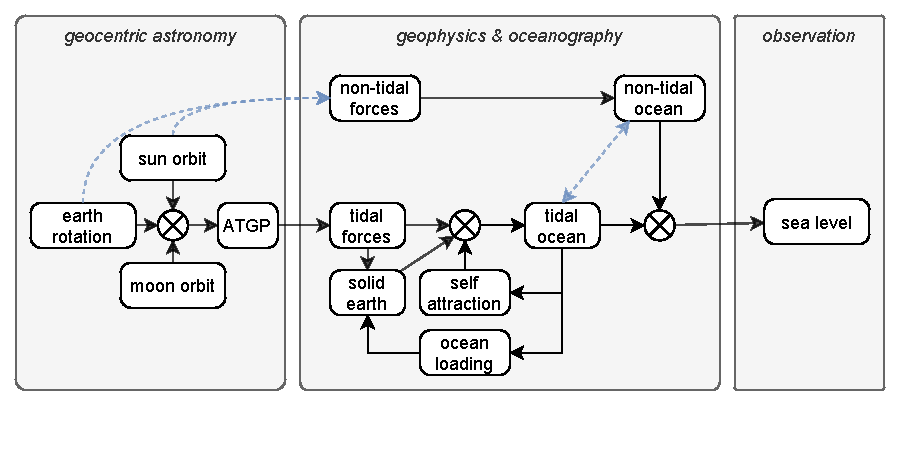
\includegraphics[width=\figwidthFull]{figures/diagrams/tidal_force_flowchart.pdf}
    \caption{Ocean tide flow chart (following Agnew \citep{Agnew:2011ub}.  Reference to the \ATGP{} is common to tidal analysis and prediction methods, whilst the treatment of tidal/non-tidal connections can differ markedly.}
    \label{fig:tideForceFlow}
    \end{center}
\end{figure}
%-----------------
Before expanding on the role of the tidal forcing, the recent work of \cite{10.1016/j.oceaneng.2020.107013} is worth mentioning.   Regardless of the finer details, this observation-based machine learning application to tide prediction is still founded on the connection between positional astronomy and sea level, but simply makes the connection more indirect by relying on easily accessible moon phase data.
%-----------------i
\subsection{Basic development of the \ATGP{}}  \label{sec:basic_potential}
The centrality of the tidal generating potential to sea level forecasting warrants further elaboration, in order to later explicate the manner in which conventional and dynamic sea level forecasts respectively represent tides. 

The \ATGP{} is a mathematical abstraction founded on a consideration of the classical gravitational field near the Earth surface. The temporal variations of gravity in the vicinity of this surface are developed as a function of the \emph{geocentric} relative positions of the celestial bodies.
For ocean tide applications, only the two celestial bodies, the moon and sun, are considered relevant on the basis of relative contribution to the perceived gravity field changes. It follows that the information required for computation of this lunisolar tidal potential is encapsulated in the celestial positions (ie ephemeris) of the moon and sun alone \citep{Agnew:2011ub}.


The full gravity field is defined as a scalar potential in space fulfilling the Laplace equation $\Delta V=0$ \citep[sec 5.3.1]{Urban:2013vl}.  The spatial field $V(\theta,\lambda,r)$ can be formulated in spherical geocentric (ie fixed earth) coordinates as a weighted sum of surface spherical harmonics. As a potential field, contributions from each mass element can be computed separately and linearly superposed.

The specific subset of $V$ attributed to the celestial bodies external to the Earth, but excluding components acting uniformly over the Earth's surface, is defined to be the tidal potential \ATGP{} or $V_T$.
The associated tidal acceleration at any particular point on the earth surface can also be thought as the vector difference between the direct attraction of each celestial body and the orbital acceleration about the Earth-Body barycenter \citep{Wenzel:1997kn}.


The subset $V_T$ of $V$ that is relevant to ocean dynamics is formulated in geocentric coordinates following the convention of \cite{Cartwright:1973em} hereafter \CTE{}, and more recent notation of \cite{Desai:2006wo}:
\begin{equation}
    \eta_{eq} = \frac{V_T(t,\theta,\lambda) }{g} = \sum_{n=2}^{\infty} \sum_{m=0}^{m=n} M_{nm} P_{nm}( \sin(\theta) ) \text{Re} \left [ c^{*}_{nm}(t) e^{im\lambda} \right ]
    \label{eq:VT}
\end{equation}
Where the potential is described only on an idealised spherical earth surface in terms of time, longitude $\lambda$ and latitude $\theta$, as a sum of functions described further below. 

$P_{nm}$ are the associated Legendre polynomials of degree $n$ and order $m$.  Writing $P_{nm}(\sin(\theta))$ gives the surface spherical harmonics.  The fact that the sum begins at $n=2$ is discussed below.
$M_{nm}$ are normalisation factors, that whilst not of direct interest here are noted to follow different conventions between applications \citep{IERS2003}.
Figure \ref{fig:VTmaps} provides a visualisation of the field and a decomposition into spherical harmonics a single snapshot in time.
%-------------------------------
\begin{figure}[h]
    \begin{center}
    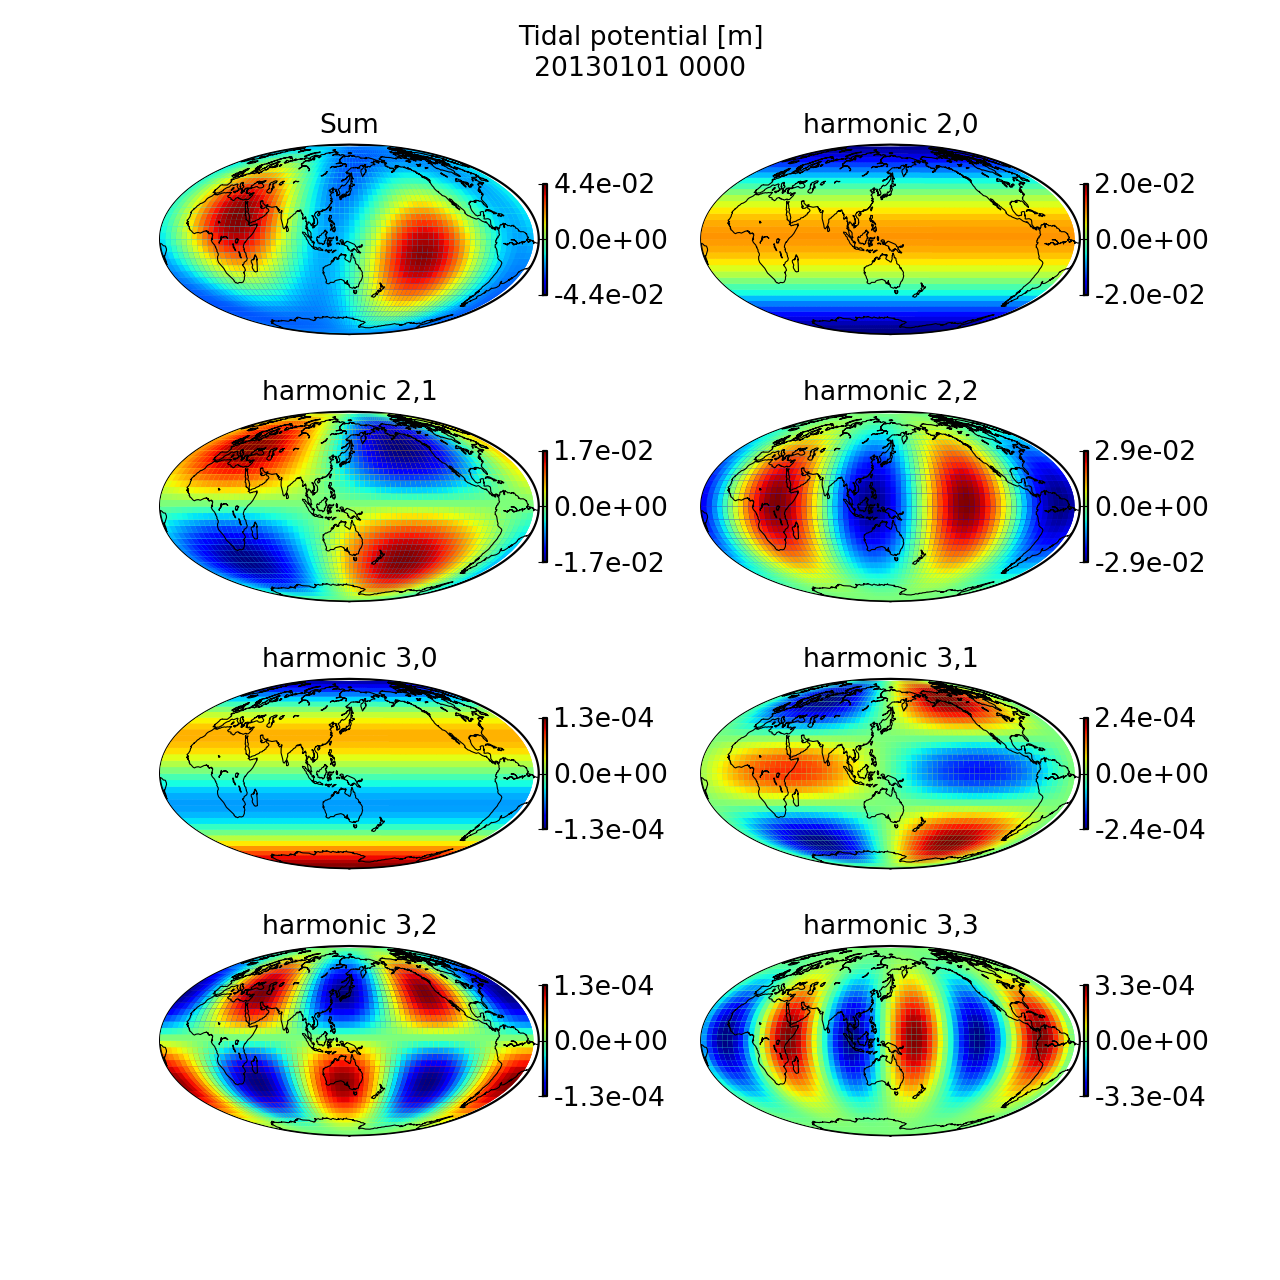
\includegraphics[width=\figwidthBig]{figures/maps/tidal_potential_spatial_20130101_0000.png}
    \caption{Snapshot of global $\eta_{eq}$ field illustrating spatial decomposition into spherical harmonics.  Note the wide variation of relative magnitude. When comparing to formulations recall that those decompositions are per body; ie an independent set for the moon and sun. }
    \label{fig:VTmaps}
    \end{center}
\end{figure}
%-------------------------------
Equation \ref{eq:VT} and the visualisation in \ref{fig:VTmaps} quantify the potential $V_T$ normalised by the standard value for Earth gravity $g$; a quantity defined as the \emph{equilibrium tide} $\eta_{eq}$.  
A convenience of normalising the potential field as $\eta_{eq}$ is that the quantity has units of height. But this formulation unfortunately invites confusion with actual ocean elevations; whereas the equilibrium tide really only has a very abstract and indirect connection to observed ocean tide heights.
Specifically, whilst useful for formulating the driving force, the any direct connection to ocean response is only via the thought experiment of a shallow water idealisation of boundary-free ocean with ``no dynamic effects'' as stated by \cite[Eq 9.8.3]{gill1982atmosphere}; that is, the equilibrium tide is a useless approximation to ocean heights at all expect the longest periods \cite{Egbert:2003jd}.


Equation \ref{eq:VT} represents the spatial decomposition of a surface potential field over the globe.  Of itself, such a formulation asserts nothing specific about the causation of the field.  It embodies no astronomy or ocean dynamics.
Practical implementation of \ref{eq:VT} requires choices regarding the set of harmonics $(n,m)$ to be included and the determination of the time varying complex weights $c_{nm}(t)$.


Only a small set of $(n,m)$ is taken to be relevant for ocean tidal dynamics; in contrast to the thousands of terms utilised for some earth gravity studies. What counts as a relevant ocean subset is generally determined on the basis of the relative magnitude of the terms and the nature of the temporal variation in geographic coordinates.

It is only the horizontal gradient of the potential $\nabla V_T$ that can drive changes in the distribution of ocean mass.   Which to be clear states that the effect of the \ATGP{} on the ocean is to slide mass side-to-side, not directly pull it up.   And furthermore, only \emph{temporal} changes in this horizontal gradient will effect the non-static ocean distribution. Subsequently degrees $n=0,1$ are not relevant to ocean tides.   This is represented in equation \ref{eq:VT} by the lower limit $n=2$ of the outer sum.
For almost ocean tide applications an upper limit of $n=2$ is taken to be sufficient, or at most $n=3$; again in contrast to some earth gravity studies.  This choice is based on the rapid decline in relative magnitude of each harmonic with increasing $n$ for the luni-solar system - discussed below regarding equation \ref{eq:c}.



The zonal harmonics $(n,m) = (2,0)$ for each body are of particular relevance to the slower patterns of sea level.  Specifically, by having no variation in $\lambda$ these harmonics don't vary geographically with the daily rotation of the earth.   However, the slower changes in the declination of each body do drive an ocean mass response and is associated with the both the long period and permanent tides.  
What is considered to comprise the \emph{permanent} component of the tide potential is effectively time scale and application dependant and is an important detail for geodesy and gravity studies.  \cite[section 5.3.3.2]{Urban:2013vl}.  For ocean forecasting, the role and formulation of the permanent tide becomes relevant in the decomposition of mean sea level, and estimation of what constitutes dynamic ocean topography in a consistent geodetic reference framework \citep{Filmer:2018cu}\cite{10.1007/bf02520477}.


All of the temporal variation of $V_T$ is contained in the time series of complex scalar weights $c_{nm}(t)$.
It is significant that these temporal variations of the \ATGP{} for the entire globe can thus represented by a small number of scalar timeseries - a single complex timeseries for each spherical harmonic included.  For the typical set of harmonics used for ocean tides $(n,m)=(2,1),(2,2)$ this represents a significant compression of spatial information.  
Given the positions in the geocentric reference frame $\theta,\lambda,r$ for both moon and sun, the coefficients are:
\begin{align}
\label{eq:c}
c_{nm}(t) &= a_{nm}(t) + ib_{nm}(t) \nonumber \\
          &= \sum_{b=\text{moon},\text{sun}}    \frac{4 \pi GM_{b}}{g r_{b}}  \frac{(2-\delta_{m0})} {(2n+1)} \left(\frac{a}{r_b} \right)^n    M_{nm} P_{nm}( \sin(\theta_b) ) e^{im\lambda_b}
\end{align}
The normalisation used in the determination of $c_{nm}(t)$ must be consistent with that used for equation \ref{q:VT}.
Note that $\theta,\lambda$ in Equation \ref{eq:c} are equivalent to the geographic coordinates of the respective sub-body point at a given time. 
Where $\delta_m0 = 1$ for $m==0$ and $\delta_{m0} = 0$ for $m \neq 0$.\\
Normalisation $M$ is given by Equation \ref{E:M}. The radial scale $a$ is conventional taken as the semi-major axis from the ellipsoidal georeference. 
%---------------------
\begin{figure}[h]
\begin{center}
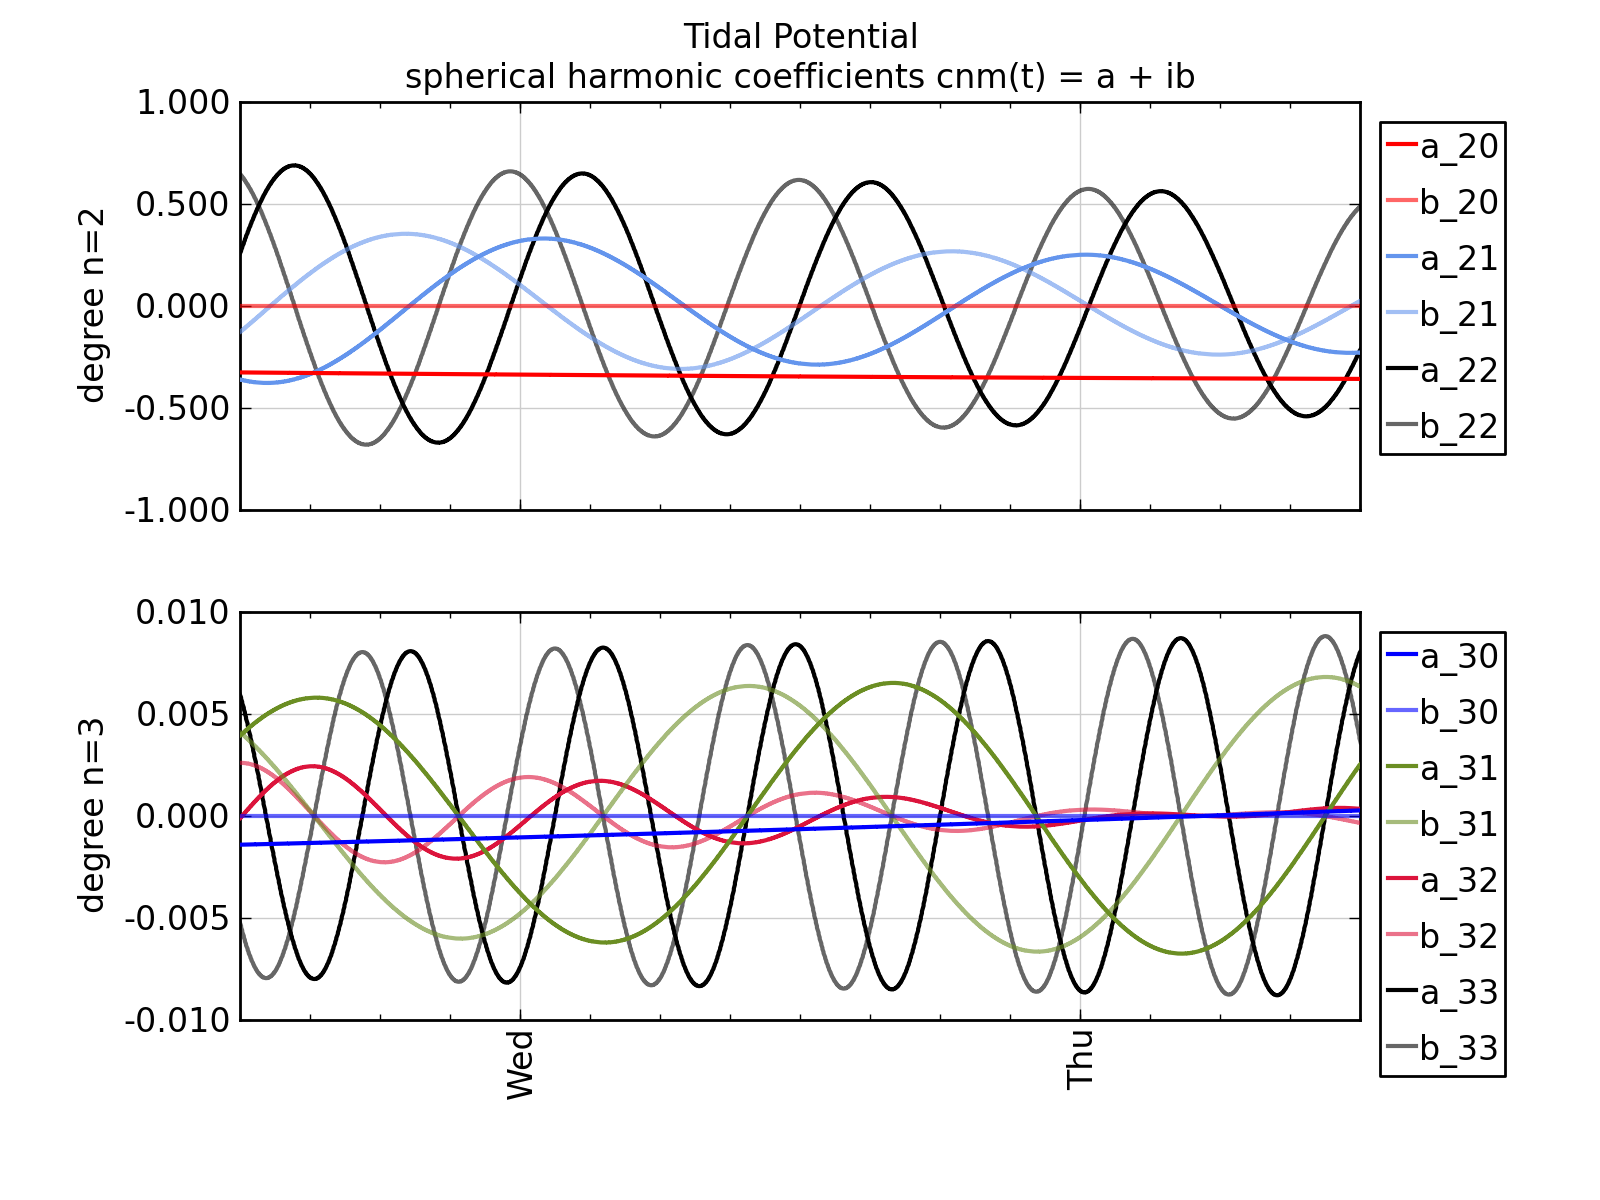
\includegraphics[width=\figwidthBig]{figures/plots/tidal_coeff_timeseries_2days.png}
\caption{Snapshot of time varying coefficients $c_{nm}(t)$.  In the upper panel, classification of $c_{2m}$ into long (red) , diurnal (blue) and semi-diurnal (black) species is evident.  Note the much smaller magnitude of higher degree harmonics.}
\end{center}
\end{figure}
%---------------------
The rapid decay of the scaling term $\left(\frac{a}{r_b} \right)^n$ with n is the basis for excluding higher degree harmonics from ocean tide applications.  In the case of the Moon, the magnitude of the $n=3$ potential field is more than 2 orders of magnitude smaller than $n=2$.  The associated force also decays, but not quite so rapidly due to the decreasing spatial length scales of the higher harmonics.  This decay is apparent in the colorbars of Figure \ref{fig:VTmaps}\\
The same relative magnitude argument is applied to neglecting more distant celestial masses from formulation of $\eta_{eq}$.

%-----------------%
\subsection{Primary role for temporal variations}
\label{sec:temporal}
The temporal variation of the \ATGP{} is of special relevance to ocean tide prediction.  And inspection of equation \ref{eq:VT} show that all of this variability is contained within the coefficients $c_{nm}(t)$.  
Any tidal method that applies $c_{nm}(t)$ from a numerical ephemeris in time-space could be said to be \emph{direct}. 
However, transformation of $c_{nm}(t)$ into frequency-space is in fact the basis of many tidal methods.   The highly clustered frequency content of $c_{nm}(t)$ renders this transformation particularly useful.  
Transformation of $c_{nm}(t)$ into frequency space is the basis for \underline{harmonic developments} of the \ATGP{}. Whilst there have been different approaches to performing this development, the common representation is given in Equation \ref{E:harmonic} following \citep{Desai:2006wo} and \citep[Eq 13]{Cartwright:1971iz}.
Furthermore, the ephemeris details for the celestial bodies can be modelled with relatively simple polynomial functions of time; discussed further below. 


It is this harmonic decomposition of the \ATGP{} that leads to the conventional ocean tide practice of harmonic analysis.
%----------------
\begin{equation}
    c_{nm}(t) = \sum_{k} H_{nmk} e^{-i( t\theta_{nmk})} = \sum_{k} H_{nmk} e^{-i( t\omega_{nmk} + \beta_{nmk})}
    \label{E:harmonic}
\end{equation}
%----------------
The index $k$ represents a discrete series of tidal components; potentially expanded out to hundreds of terms.  Each component is associated with a discrete point in complex frequency-space with amplitude $H$, frequency $\omega$ and phase $\beta$.

Despite a common misconception, it is important to emphasise that equation \ref{E:harmonic} does not represent a Fourier series.  The finite sequence of frequencies $\omega_{nmk}$ are derived from the relative motions of the earth-moon-sun system and do not provide either an orthogonal set of sinusoids nor a complete basis.

Despite not being orthogonal, the harmonic decomposition does provide a special list of frequencies that can be ranked by a scalar magnitude. 

\citet{Doodson:1921kt} introduced a novel and influential system of notation for specifying $\theta_{nmk}$ based on a laborious harmonic decomposition of $V_T$ using Brown's lunar theory; that is, a polynomial model for the lunar ephemeris.  
In the Doodson formulation, all the relevant astronomical information is summarised by code of 6 small integers; together called the Doodson number or argument numbers.   Each position in the code is associated with an fundamental astronomical concept as summarised in Table \ref{T:doodson}.  Doodson codes are in common use across the tidal literature and provide the only useful means of describing tidal components beyond the small number associated with traditional Darwin names such as M2, K1, O1, S2.
Of these traditional names \citet{10.1016/b978-0-444-53802-4.00058-0} correctly states that `` [whilst] it is convenient to have a shorthand way of referring to these harmonics; unfortunately, the standard names,  now totally entrenched, ... simply have to be learned as is.''.

There has been some variation of conventions with regard to the exact formulation of Doodson numbers.  One such detail is the avoidance of negative integers in the code by the addition of the arbitrary constant 5 to all integers except $d_1$.   A less common variation involves the use of solar-hour in place of lunar hour $\tau$.  
In essence the Doodson codes provide a compact unique specification, or in practice \emph{definition} of frequencies relevant to tidal methods.

Whereas the Doodson codes provide a reliable way to describe these tidal frequencies, the mapping to traditional names is unfortunately not always consistent and can lead to errors if transferring parameter data between software platforms; this issue is taken up in chapter \ref{chp:tideFlavours}.


\begin{table}[htp]
\caption{Doodson astronomical arguments.  Small integer combinations of these six numbers $d_1 d_2 d_3 d_4 d_5 d_6$ are used to classify tidal components.  Recall that longitudes are celestial, not geographic, coordinates}
\begin{center} 
\begin{tabular}{|c|c|c|}
\hline
Description                            & Argument          & Period\\
\hline
Mean lunar hour                        & $\tau$            & $\sim$ 1 day      \\
Moon mean longitude                    & $s$               & $\sim$ 27 days    \\  
Sun mean longitude                     & $h$               & $\sim$ 1 year     \\
Longitude of lunar perigee             & $p$               & $\sim$ 8.85 years \\
Negative longitude of mean lunar node  & $N^\prime$        & $\sim$ 18.6 years \\
Longitude of Sun mean perigee          & $p_1$             & $\sim$ 20000 years\\
\hline
\end{tabular} 
\end{center}
\label{T:doodson}
\end{table}


Equation \ref{E:doodson} gives the angular argument for a single tidal component $k$ as a function of the 6 astronomical arguments.   As discussed above, the astronomical arguments embody an analytical ephemeris for the Moon and Sun rather than a direct numerical description of these positions.  Polynomial functions of time can be used to estimate each of the 6 arguments close to a given epoch.  The phase adjustment $\delta$ is a convention applied such that the each term in \ref{E:harmonic} is written as a cosine, rather than the mixture of sine and cosine terms that naturally follow from the underlying spherical harmonics.

\begin{align}
\label{E:doodson}
\theta_{nmk}  &= \left[ d_1 , d_2 , d_3 , d_4 , d_5 ,d_6 , \delta(n,m)  \right] \cdot \left[ \tau , s  , h , p , N^\prime , p_1 , \frac{\pi}{2}   \right]   \\
          d_1 &\equiv m \nonumber \\
              & \mbox{ (nb ignoring integer offset 5 often added to $d_2d_3d_4d_5d_6$)} \nonumber
\end{align}

\begin{equation}
\delta(n,m)  =     \begin{array}{ll}
                    1 & \mbox{if $n+m$ odd}  \\
                    0 & \mbox{if $n+m$ even} 
                    \end{array}             
\end{equation}


%-----------------%
\subsection{Other aspects relevant to global coordinates}
\label{S:ATGP_extras}
The essential development of the \ATGP{} in Section\ref{sec:basic_potential} is standard.  However, progressing beyond the basic development towards an ocean forecasting application raises several issues of significance that depend on the details of the application.\\


\underline{Solid Earth deformation and vertical reference.}  \\
The basic spatial perspective behind the development of the \ATGP{} is the thin shell approximation.  Geocentric coordinates are used.  This is appropriate for writing the potential in general form.  However, when considering the response of ocean dynamics, a vertical relative to the ocean floor is dynamically relevant.  There is a vertical movement of the ocean floor in geocentric coordinates associated with the \ATGP{} of comparable magnitude to the ocean tide which is quantitatively significant to dynamic models \citep{Hendershott:1981ub} and \citep[pp.336]{gill1982atmosphere}.\\
This elastic response of the earth can considered to be essentially instantaneous compared to ocean timescales.  Furthermore, the elastic re-distibution of mass associated with this 'earth tide' itself modifies the gravitational field.    By treating the Earth as "spherical, non-rotating, elastic, and isotropic" the solid body response can be encapsulated by a small number of dimensionless Love numbers \citep{Agnew:2011ub}.  In the present context each spherical harmonic degree has a single body tide Love number $h_n$ and `induced free space potential' Love number $k_n$ \citep[Sec 5.3.3]{Urban:2013vl}. This has the convenience of formulating the combined \emph{direct} effects of the solid earth response to the \ATGP{} as a modification to the magnitude of $\eta_{eq}$.  It is noted that ``the Love numbers for the diurnal tides differ from those for the semi-diurnal and long-period tides because of the free-core nutation resonance'' \citep{Arbic:2004wz}.\\
The conceptually related, but more complicated, effects of the moving ocean mass itself is discussed below.

\begin{equation}
\eta_{eq} = -(1+k_n-h_n) \frac{V_T}{g} \sim 0.7 \frac{V_T}{g}
\end{equation} 



\underline{Treatment of self attraction and loading.} \\
The tidal movement of ocean mass has an effect on the solid Earth, and reflexively on the gravitational potential acting on the ocean itself.\\
From an ocean modelling perspective, elastic compression of the solid earth due to the time varying mass of ocean is referred to as the `load tide'.  The effect of the moving distribution of ocean mass on the gravitation potential field is referred to as `self-attraction'.\\
Together these effects are lumped together as self-attraction and loading \SAL{}.  They are conceptually distinct from body tides in that \SAL{} is a reflexive function of the time varying spatial distribution of global ocean mass.\\
Similar effects that vary on tidal timescales are also associated with the time varying distribution of atmospheric mass as well land-based loading from ice,snow and soil moisture.  The value of explicitly distinguishing non-ocean \SAL{} in the context of ocean forecasting is not known, and no publications appear to address this in detail.  It is likely that practical evaluation of \SAL{} for ocean modelling implicitly accounts for some atmospheric effects - especially for the ocean tide associated with pressure forcing S1 and S2.\\



Similarly to body tide effects, it is possible to formulate \SAL{} as a scaled modification to the \ATGF{}.  This is very convenient, but known to be associated with significant inaccuracies \citep{Ray:1998jl}.  The present distribution of \MOM{} makes this so called `$\beta$' approximation.\\
An evaluation of intermediate methods to parameterise SAL is described by Stepanov and Hughes \cite{Stepanov:2004up}
In contrast to the $\beta$ scaling approximation, it appears to be quite reasonable to consider \SAL{} as separate pre-calculated body forcing rather than a scaling of $\eta_{eq}$. 
\begin{quotation}
SAL should be computed by convolution \dots with the Green's function for loading and self-attraction. Since this convolution smoothes out small-scale features, and since large-scale tidal elevations are now well determined over most	of the earth, SAL is in fact now reasonably well known, even where local details of tidal elevations and currents remain uncertain. \citep{Egbert:2002ug}
\end{quotation}




\underline{Time, polar motion and ephemeris.}\\ 
Diurnal Earth rotation and hence time UT1 are effected by tidal effects \citep[sec 8]{Anonymous:2004tm}.  In addition, conventional UT1 contains discontinuities at leap seconds is not strictly identical to ephermeris time.  For the purposes of ocean forecasting these variations are in general considered negligible and definitions of time are treated as unproblematic.\\




A special case is the \underline{pole tide}. Geocentric coordinates align the polar zenith approximately with the Earths axis of rotation. However, there are continual variations of alignment from the reference axis described by theories of precession and nutation and in general referred to as `polar motion'.   More generally, any changes in the Earth's instantaneous rotation vector can be associated with changes in the gravity field  experienced in surface fixed geocentric coordinates.\\
\begin{quotation}
Polar motion of the Earth is almost completely described by two harmonic variations of the location of the instantaneous rotation pole with respect to the mean rotation pole: an elliptical motion at an annual period, and an almost circular motion at a period of 14 months. The 14-month variation is a free mode of the Earth referred to as the Chandler wobble and has amplitudes that vary with time. \citep{Desai:2002ev}
\end{quotation}
The gravitational effect due to polar motion can be formulated similarly to the \ATGF{} as a potential field decomposed into spherical harmonics.
Pole tide effects are included as corrections to altimetry products, but are ignored in standard tide table production.\\
Another phenomena effecting Earth rotation is the Free Core Nutation (FCN).  For the present ocean tidal purposes the FCN will be considered relevant only with regard to the solid earth tides.  The FCN is a factor in defining the  Love numbers in the diurnal band.   Related to this, Desai and Wahr note that the definition of the K1 $[1 1 0 0 0]$ input amplitude used for solid earth tide algorithms can be inappropriate for ocean applications if compensation for the effects of the FCN resonance are included\cite{Desai:1995je}.



The formulation of the tidal potential in Section\ref{sec:basic_potential} involved only the instantaneous relative positions of the Earth-Moon-Sun system.   These positions are taken from an ephemeris.  In practice, there are two broad classes of ephemeris; analytical and numerical \citep{Wenzel:1997kn}.


An analytical ephemeris provides the relative positions of the Moon and Sun via relatively simple polynomial relations, optimised for a given epoch.  Such analytic ephemeris have been commonly employed for ocean tide studies.   Analytic ephemeris were used initially for computational necessity and more recently for computational convenience.


For modern \emph{astronomical} purposes numerical ephemerides are now standard.  Prior to 1984 standard ephemeris were based upon \emph{theories}\cite[sec 8.1]{Urban:2013vl}, whereas contemporary ephemeris are created by the application of dynamical equations integrated into the future, after initialisation via assimilation of past observational data.

At the time of writing, the current best estimates for the orbits of the Moon and planets is DE421 \citep{Folkner:2008wm}.   The snapshot visualisation shown in Figure \ref{fig:VTmaps} were calculated based on the application \ref{eq:c} to output of DE421.


The direct application of modern numerical ephemeris to global ocean tide simulations has been demonstrated by for instance \cite{Weis:2008ex} and \cite{10.1007/s10236-016-1016-1}.
However the attractive properties of this approach appear yet to have outweighed the benefits of conceptual and implementation simplicity offered by conventional decomposition approaches.   The ability to isolate named constituents for evaluation is valued for inter-comparisons such as that of \cite{Stammer:2014vh}
A more accurate ephemeris is likely of less significance to ocean tide hydrodynamics than the conceptual approach regarding the extent to which forcing and response are viewed in frequency space \citep{10.17125/gov2018.ch13}.

Considering the ocean response to tidal forcing in frequency-space is arguably just as foundational to tide prediction and sea level studies as the \ATGP{}; and this topic is addressed next.  

%-----------------%
\subsection{Ocean as an LTI System}
\label{sec:LTI}
With historical hindsight it could be said that the success of tidal sea level prediction have been based on treating the ocean as a linear time invariant (LTI) system driven by the \ATGP{}.\footnote{The nomenclature LTI is taken from engineering control theory , and not the historically influential Liverpool Tide Institute.}

In essence, the ocean response to tidal forcing is modelled as stationary in frequency space.  Once this time-invariant ``black box'' model has been characterised, astronomical empherides map linearly to sea level predictions.  The details of how the LTI system is characterised and implemented distinguish the variants of tidal analysis and prediction.

Two important aspects of this broad approach were introduced in the late 1700's by Laplace \cite[chpt 7]{Cartwright:2000tt}:
\begin{itemize}
    \item the spectral banded-ness of $V_T(t)$ and the value of a stationary frequency perspective;
    \item application of semi-empirical analysis to simply characterise the expression of complex hydrodynamics. 
\end{itemize}

Modelling the ocean as an LTI system in this manner necessarily takes a frequency-space perspective and assumes model stationarity. \citet{Jay:2003bj} suggest that that the long history and apparent value of this perspective has $\dots$
\begin{quotation}
solidified an opinion that tidal time series (particularly those of surface elevation) are basically stationary, with non-stationary components frequently being regarded as meaningless `noise'.    
\end{quotation}
In fact, as discussed in section \ref{sec:semantics}, frequency-space stationarity is essential to the \emph{definition} of what is considered tidal in most operational settings.
% little flow chart
\begin{align}
    c_{nm}(t) \Rightarrow & \fbox{Global Ocean}\Rightarrow \mbox{observed response} \nonumber
\end{align}

Time invariance of the LTI in frequency-space means that each input component maps directly to an output response at the same frequency, characterised by an amplitude and phase transformation.   As the LTI characteristics are identified via semi-empirical methods, any hydrodynamics are essentially hidden within the black box and are largely irrelevant.

The core of such a tidal model is schematically shown as a mapping at each distinct tidal frequency:
\begin{align}
    H_{k}(\theta_k) \Rightarrow & \fbox{empirical LTI system} \Rightarrow \mbox{tidal ocean $f(\theta_k)$}  %\nonumber
    \label{eq:LTI}
\end{align}

Conceptualising the global ocean in frequency space raises some peculiarities as characterised by  \citet{Groves:1975ky}: ``by an unfortunate coincidence, the size of the earth, the depth of the ocean, and the rate of earth rotation are such that the frequencies of the free modes of ocean oscillation are intercalated with the frequencies of the tide-generating consitituents''.
For sea level, the different forecasting methods are essentially variants on the  definition of a reference input signal and manner in which the LTI system is formulated.   Following Munk and Cartwright \citep{Munk:1966ts} there are three foci for the problems associated with this conceptualisation:
%\begin{inparaenum}[(i)]
\begin{itemize}
\item the spectral continuum of ocean variation;
\item non-gravitational phenomena; 
\item non-linear interactions.   
\end{itemize}
%\end{inparaenum}

%-----------------%
\subsection{Tidal Harmonics and Formalisms}
\label{sec:formalisms}
There is no unique approach to implementing the LTI concept of ocean tide prediction. In fact, ``\textit{many organizations have developed their own methods of tidal analysis}''\citep{IOC:2005tj}. But the different approaches or formalisms share the LTI system model discussed above.  
In very broad terms tidal these formalisms fall into basically two categories: harmonic methods and response methods.  
Neither of these concepts actually involve any hydrodynamics. When hydrodynamic simulations of the ocean are undertaken it seems that tidal LTI conceptualisations are at least indirectly involved in one way or another; and this will be apparent in subsequent sections dealing with hydrodynamic and spatial models. 

Within operational authorities, \emph{tide prediction} is practically synonymous with conventional harmonic methods. And it is here that the role of special frequencies (section \ref{sec:temporal}) has come to play a primary role.
``Standard harmonic methods demand little accuracy in the harmonic amplitudes of the [tidal] potential, since they \textit{use only the frequencies} at which the larger amplitudes appear, and certain details on which to base nodal corrections''\cite{Cartwright:1973em} emphasis added.
Recall that the basis for this analysis is not harmonic in the sense of an orthogonal Fourier series, but rather that it follows from the harmonic development of the \ATGP{} as described in section \ref{sec:basic_potential}.    Here again the historical legacy of tidal terminology lends itself to misunderstanding \citep{Cartwright:2000tt}\citep{Parker:2007wq}.


Harmonic methods of sea level prediction are very successful and will continue to be important for years to come, regardless of other advances.  The conventional and routine harmonic analysis of tide-gauge data provides a foundational set of products that is embedded across the whole coastal economy. Tide tables and derived tidal planes (such as LAT) provide ubiquitous references for both land and marine applications. This situation provides some of the difficulties discussed in Chapter \ref{chp:aggregate}, and is elaborated further in  Chapter \ref{chp:tideFlavours}.


At its foundation, harmonic tidal analysis and prediction characterises the ocean response as a LTI system via a finite set of amplitude and phase terms that are identified empirically by the application of timeseries methods.   This concept is stated a little too simply in the Australian Tide Manual as follows: ``\textit{ the purpose of tidal analysis is to represent the water level or current time series by a set of harmonics, or sine waves, each of them having a specific amplitude and phase}''\citep{PCTMSL-sp9}.
Note the emphasis on periodicity rather than dynamics.  More problematic is the fact that this stated purpose is neither universally agreed nor implemented by any tidal agency, as the following discussion will outline.  
The conventional harmonic tide representation of a timeseries is given in equation \ref{eq:cos}.  At face value involves a linear sum of sinusoids with amplitude $A_k$ and phase lag $g_k$ parameters considered to be constants that characterise the LTI system; other terms and complications are discussed below.  
%---------------------
\begin{equation}
\eta_{tide}(t) = \sum_{k} f_k A_k \cos ( t.\omega_k + g_k + u_k)
\label{eq:cos}
\end{equation}
%---------------------
Significantly, the harmonics involved with such an analysis can only ever be a \emph{subset} of tidal frequencies arising from the decomposition $c(t) = \sum_{k} H_{k} e^{-i( t\theta_{k})}$.  This limitation comes mainly from the non-orthogonality of the basis functions and the fact that all observational records are of finite length.
Conventional tide practice applies a range of elaborations and work-arounds in order to select the set of analysed components and produce predictions.  
Before discussing any further, the essential steps of the harmonic analysis and prediction process are  illustrated schematically in Figure \ref{fig:tidePractice} and summarised as follows:
\begin{enumerate}
    \item formulation of component set based on various conventions;
    \item empirical projection of an observation record onto the resulting non-orthogonal basis functions;
    \item application of conventions accounting for unresolved frequencies; 
    \item synthesis of tidal timeseries by applying matching conventions.
\end{enumerate}

The practical value of harmonic methods reflects the special significance of sea level variation occurring at tidal frequencies. This value does not rely on simulating ocean dynamics. Rather, the very \emph{absence} of fluid dynamics is a key strength of harmonic methods. 
A record of historical observations at one place is essentially all that is required, with no need for spatial information or any additional inputs whatsoever.

For almost all ocean-exposed locations, harmonic analysis can reduce the majority of sea level variance in a long observational timeseries to a remarkably short list of numbers; typically mapping several thousand values to a few dozen \citep{Flinchem:2000kp}.  This unique data compression could be better exploited for on-demand delivery services as suggested in chapter \ref{chp:tideFlavours}. 


The standout power of some tidal variations is apparent in the spectra shown in Figure \ref{fig:obsSpectraEg}. 
But conventional practice has developed additional terms that are not directly apparent in the \ATGP{} that have in some locations greatly improved the value of the resulting predictions; in particular for what are called the compound, shallow water or overtide terms. In this cases, hydrodynamic reasoning has been applied to select and justify additional terms that could result from the behaviour of depth limited waves and wave-wave interactions.
Any seasonal modulation terms are analogous in the sense that the rational for the LTI model has been extended to account for observed patterns rather than derived solely from the \ATGP{}.
%----------------------
\begin{figure}[H]
	\centering
	\begin{subfigure}[t]{\figwidthHalf}
	    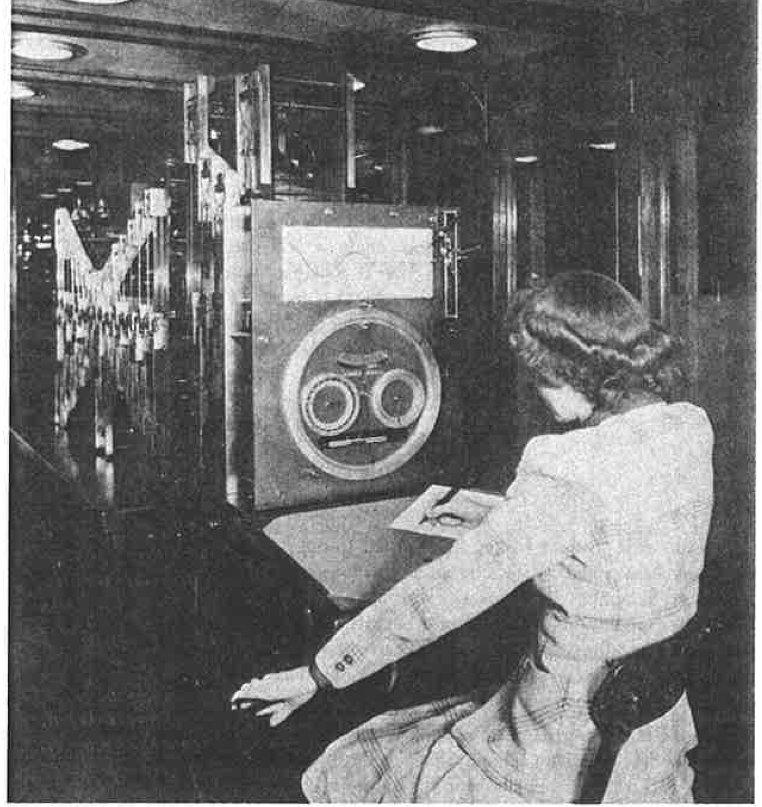
\includegraphics[width=\textwidth]{figures/images/zetler_tidal_computer_lady_1921.png}
	    \caption{Harris-Fischer tide machine circ. 1912 \protect{ \citep{Parker:2007wq} }}
    \end{subfigure}
    \hfill
    \begin{subfigure}[t]{\figwidthHalf}
    	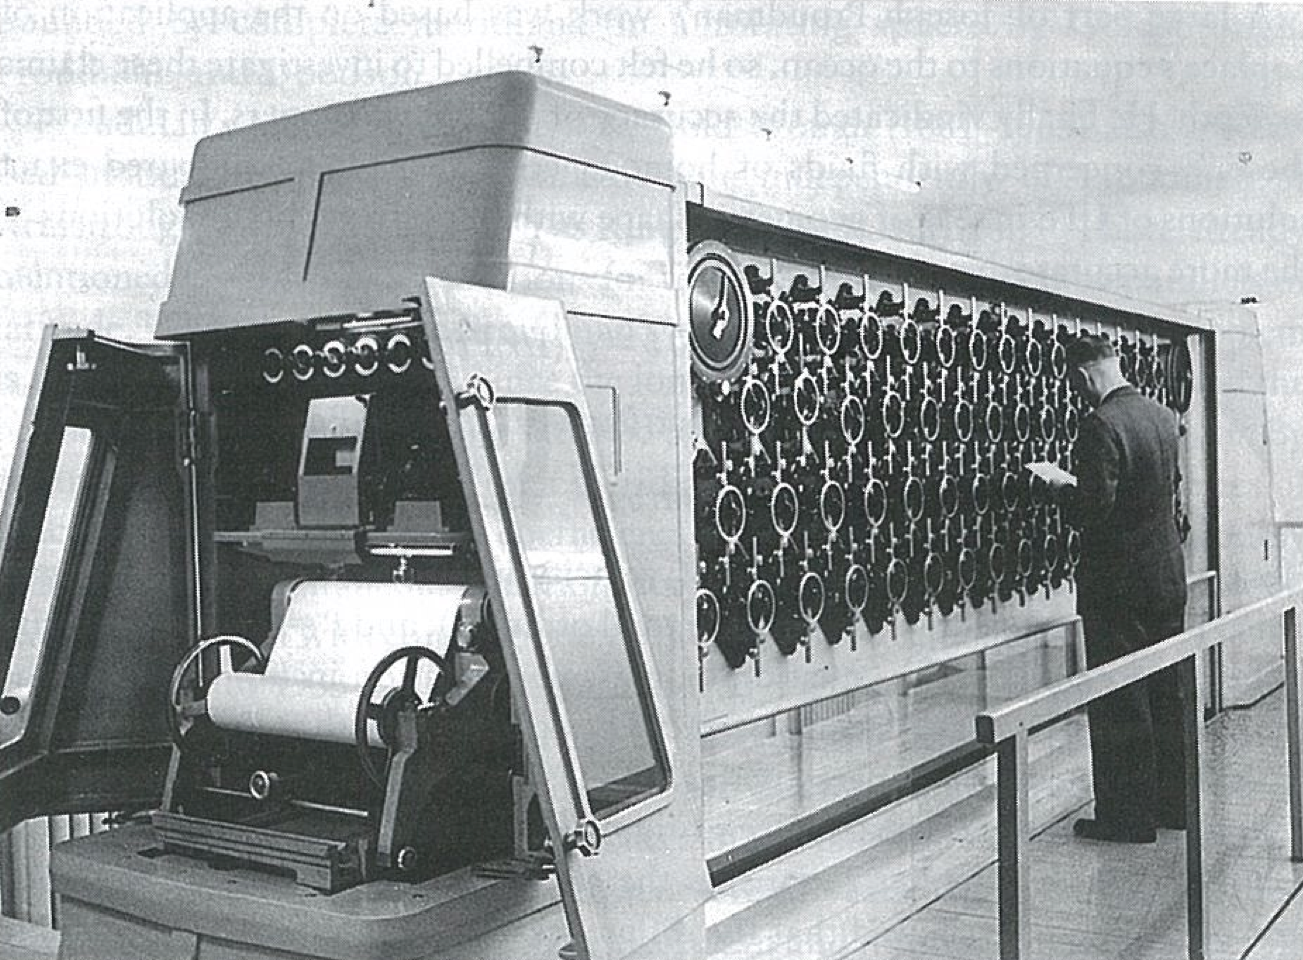
\includegraphics[width=\textwidth]{figures/images/DHI_machine_cartwright_fig11p2.png}
	    \caption{Gezeitenrechenmaschine at DHI circ. 1940 \protect{ \citep{Cartwright:2000tt} }}
	\end{subfigure}
	\caption{Analogue tide machines embody harmonic prediction.  A finite set of phase and amplitude values are dialled up and the handle turned to generate a prediction timeseries.}
	\label{fig:tide_machines}
\end{figure}
%----------------------
Harmonic analysis can be formulated as an over-determined inverse problem:
%--------------------
\begin{equation}
    \label{E:Axb}   
    \M{A} \V{x}=\V{b} 
\end{equation}
%--------------------
Where $\M{A}$ is a matrix of tidal timeseries basis functions, $\V{x}$ is the analysed tidal solution and $\V{b}$ is an observational record. The tidal basis functions are developed from the combination of the harmonic decomposition of $\eta_{eq}$ and a series of conventions.  The resulting basis is neither orthogonal nor complete. Inclusion of the modulation terms $f_k$ and $u_k$, discussed below, means that the basis functions are not actually sinusoids. The core assumption of stationarity for the finite series of basis functions is equivalent to an assumption that the basis has infinite span in time.   

Practical applications of the harmonic formalism has largely evolved prior to modern cheap computing, and many details can appear somewhat baroque in isolation.  The analogue instruments shown in Figure \ref{fig:tide_machines} serve to highlight this operational history.


The harmonic idealisation effectively operates on infinite basis functions whereas any observational record is of finite length.
Given the close clustering of tidal lines in frequency-space, equation \ref{E:Axb} is poorly conditioned for inversion.   This matrix condition is further degraded by the presence of non-tidal variations. 
Subsequently, practical harmonic analysis procedures must specify which frequencies to include in the basis set and then somehow account for the effects of unresolved frequencies.

At the time of writing the Bureau of Meteorology process does not systematically account for the inversion quality with regard to signal:noise ratios as suggested by \citet{Foreman:2009bg}.
This fact contributes to the potential for overfitting or projection of non-tidal signal onto standard tide predictions discussed in chapter \ref{chp:aggregate} and \ref{chp:tideFlavours}.


When additional constants can be inferred rather than taken directly from the inverse solution, using assumed relationships from either $\eta_{eq}$ or previous or nearby analysis.




Typically arguments regarding the relative magnitude of the harmonic components of $\eta_{eq}$ are used to prioritise candidate frequencies for inclusion with respect to the observational  record length. 
By convention, the effects of clusters of unresolved tidal frequencies are represented by modulation of the basis functions in relationships assumed to map from $\eta_{eq}$.  
In equation \ref{eq:cos} these modulation terms are included as $f_k$ and $u_k$.  These terms are misleadingly known by convention as `nodal corrections', due historically to the close spectral spacing associated with the the lunar nodal regression; differences in $\omega_k$ of about $\fract{1}{18.6}$ years.     These same terms are more informatively called `satellite modulations' by some authors in recognition that the modulation of a constituent term by a very closely spaced spectral cluster arises from terms other than $d_5$. 

Importantly, this nodal modification of basis functions means that the analysis results do not simply represent amplitudes and phases for regular sinusoids.  





To the extent that the non-astronomical phenomena are regular enough to be predictably periodic, inclusion within the LTI model can be to the benefit of a tide prediction.   On the other hand, effects that are not perfectly aligned to the \ATGF{} conflict with the fundamental LTI model and necessarily present an additional risk to forecast skill.


For instance with seasonal phenomena.   The harmonic decomposition of $c_{nm}(t)$ provides two relatively tiny signals at periods of 1 and 0.5 years - conventionally termed Sa and Ssa.  Despite the small amplitudes in $\eta_{eq}$ there are powerful seasonal variations in ocean observations that project onto the Sa and Ssa tidal components.   This is well recognised and `...whether the calculated values of Sa and Ssa are used or not, becomes almost a philosophical question, based on ones application' \citep[p122]{Parker:2007wq}.   Related terms that reflect seasonal modulation of semi-diurnal components can also included be included in standard harmonic analyses (eg H1 and H2 in Foreman schedule \citep{Foreman:1977ua})\\
Perhaps more significant methodologically, is the case of diurnal and semidiurnal sea level signals driven directly by \emph{meteorology} rather than the \ATGP{}.   The tidal frequencies denoted S1 and S2 are a prominent case in point.  For instance, Ray and Ponte \citep{Ray:2003ui} evaluate \NWP{} representations of \emph{barometric} tides at these frequencies with implications for oceanographic processes.  Treatment of S1 and S2 in tidal sea level predictions is a point of difference between the harmonic and response methods.  The later going so far as to invoke a distinct input function in the form of a `radiation potential'.    The response approach is now discussed in more detail. 


% APPENDIX?


% response methods
The \underline{response method}, and it's variations, form the primary alternative to the conventional techniques of harmonic analysis.   This consists of a generalised implementation of the LTI model, in which the ocean response to \emph{any} input sequence is characterised by a stationary admittance function.  The terminology was introduced by the influential publication \citet{Munk:1966ts}.
The authors claimed to be motivated by an application of Ockam's razor to the highly evolved historical baggage of harmonic methods.   

Some more on this topic is addressed in Appendix \ref{appendix:response}, but is not essential to the flow of this discussion.


%-----------------%
%\subsection{Tidal admittances in operations}

% LTI
It should be re-iterated that at high level, the harmonic and response models contain the same core concept.   Both model the ocean as an LTI system responding to some type of tidal forcing and both contain assumptions about the smoothness of ocean admittance.  Indeed Le Provost in \citep[chpt6]{Fu:2001ub} groups both the standard harmonic and convolution formalism as instances of the `response' formalism on this basis. \\
By definition these LTI methods are aiming to represent phenomena stationary in tidal frequency-space.  Treatment of non-stationary tidal phenomena forms a scientifically important extension, eg \citep{Colosi:2006va} and \citep{Ray:2011tj}, but presently plays a very secondary role with regard to conventional sea level forecasts.\\
A point of special interest to the explicit resolution of tides within \OGCM{}s is the relatively small but observable sea level surface signatures of nonstationary internal tides.




% harmonics == admitance
Consistent with this equivalence, it is common within the literature to refer to harmonic constants \emph{as} admittances.   A harmonic constant is seen as a sample from the admittance curve at an exact frequency. For instance Smith\cite{Smith:1997ut} provides the simple conversion to sample $Z(\omega_{nmk})$ and scale by the \ATGP{} amplitude $H_{nmk}$.
Furthermore, harmonic constants remain the lingua franca of ocean tide discussions. Regardless of the detail behind any particular method, results are almost universally transformed into conventional amplitude and phase values for intercomparisons.\\
In less specialised language however, harmonic analysis is quite distinct from a response method - especially with regard to whether the outcome is a list of constants or a series of admittance curves.\\




% inference and smooth
Regardless of the method used for analysis, an expectation that admittance curves $Z(\omega)$ should not contain discontinuities or sharp changes (the `credo of smoothness') is commonly evoked to enhance the spectral content upon the \emph{synthesis} of a tidal timeseries.  Following an analysis performed to determine admittances at a relatively small number of frequencies, $Z{\omega}$ is interpolated or extrapolated in frequency-space to infer additional spectral information.   The design of such an inference process can treat frequencies on a case-by-case basis distinguishing between component admittance curves (for instance \citep[pp 268]{Fu:2001ub}).




% operations
There is an apparently wide gap between the practices of centres producing \underline{tide tables} using conventional harmonic analysis and the more varied and advanced methods used within the scientific literature and employed for global models.


The relative significance of non-linear effects between the vast open ocean and the coastal zone provides some explanation for this split.  As illustrated in Figure \ref{fig:response}, the manner in which nonlinear feedbacks are incorporated into the response formalism significantly reduces it's elegance in comparison to the purely linear application valid for blue-water tidal analysis.\\
Another factor contributing to this gap is largely cultural.
\begin{quotation}
$\dots$ the improvement in predictable variance is numerically small compared with the natural noise in sea level.   Because of this, and the fact that the Response Method is harder for a routine operator to grasp, it has never been adopted for ordinary tide-table production. It remains essentially a research tool for specialists. \citep[pp 198]{Cartwright:2000tt} 
\end{quotation}
Expanding Cartwright's explanation, the importance of robustness and intuitive error checking to routine operations should also be emphasised.  Short tables of constants are indeed physically intuitive and facilitate simple checking.   And the presentation of spatial atlases for amplitude and phase are standard.





%-----------------%
\subsection{Distinguishing forecasts and filtering}

Sea level forecasting is not the only reason for employing tidal methods in operational centres.\\
Tidal methods are employed for two broadly distinct purposes: forecasting and filtering.  And beyond the operational context even more varied tidal methods are employed for data analysis and specialised studies.\\

The distinct motivations behind producing a forecast and filtering a signal can lead to significant differences in what is defined as the tidal component of observed sea level.   Subsequently, apparently inconsistent tidal timeseries can be in simultaneous use within an operational centre.



Filtering to remove tides from an ocean signal is commonly referred to as `de-tiding'.  Filtering is a means to distinguish signal and noise.  Application of a de-tiding process categorises tidal variations as noise so as to make use of the remnant signal.   In that respect de-tiding is nominally the inverse problem to tidal analysis.   Following the discussions in Section \ref{sec:semantics}, important details regarding what should be defined as tidal then naturally depend on the context of an application.\\
Operational oceanography in the form of \BL{} relies on de-tided altimetry observations as an important assimilation constraint.   The de-tiding process has been designed to render the observations compatible with the physics of the model, with a focus on meso-scale baroclinic variability. The current configuration of \BL{} does not assimilate tide gauge data, though in principle these insitu observations could be rendered consistent via appropriate de-tiding, for example \cite{Matsumoto:2000tg}.
%-------------------------
\begin{figure}[h]
\begin{center}
    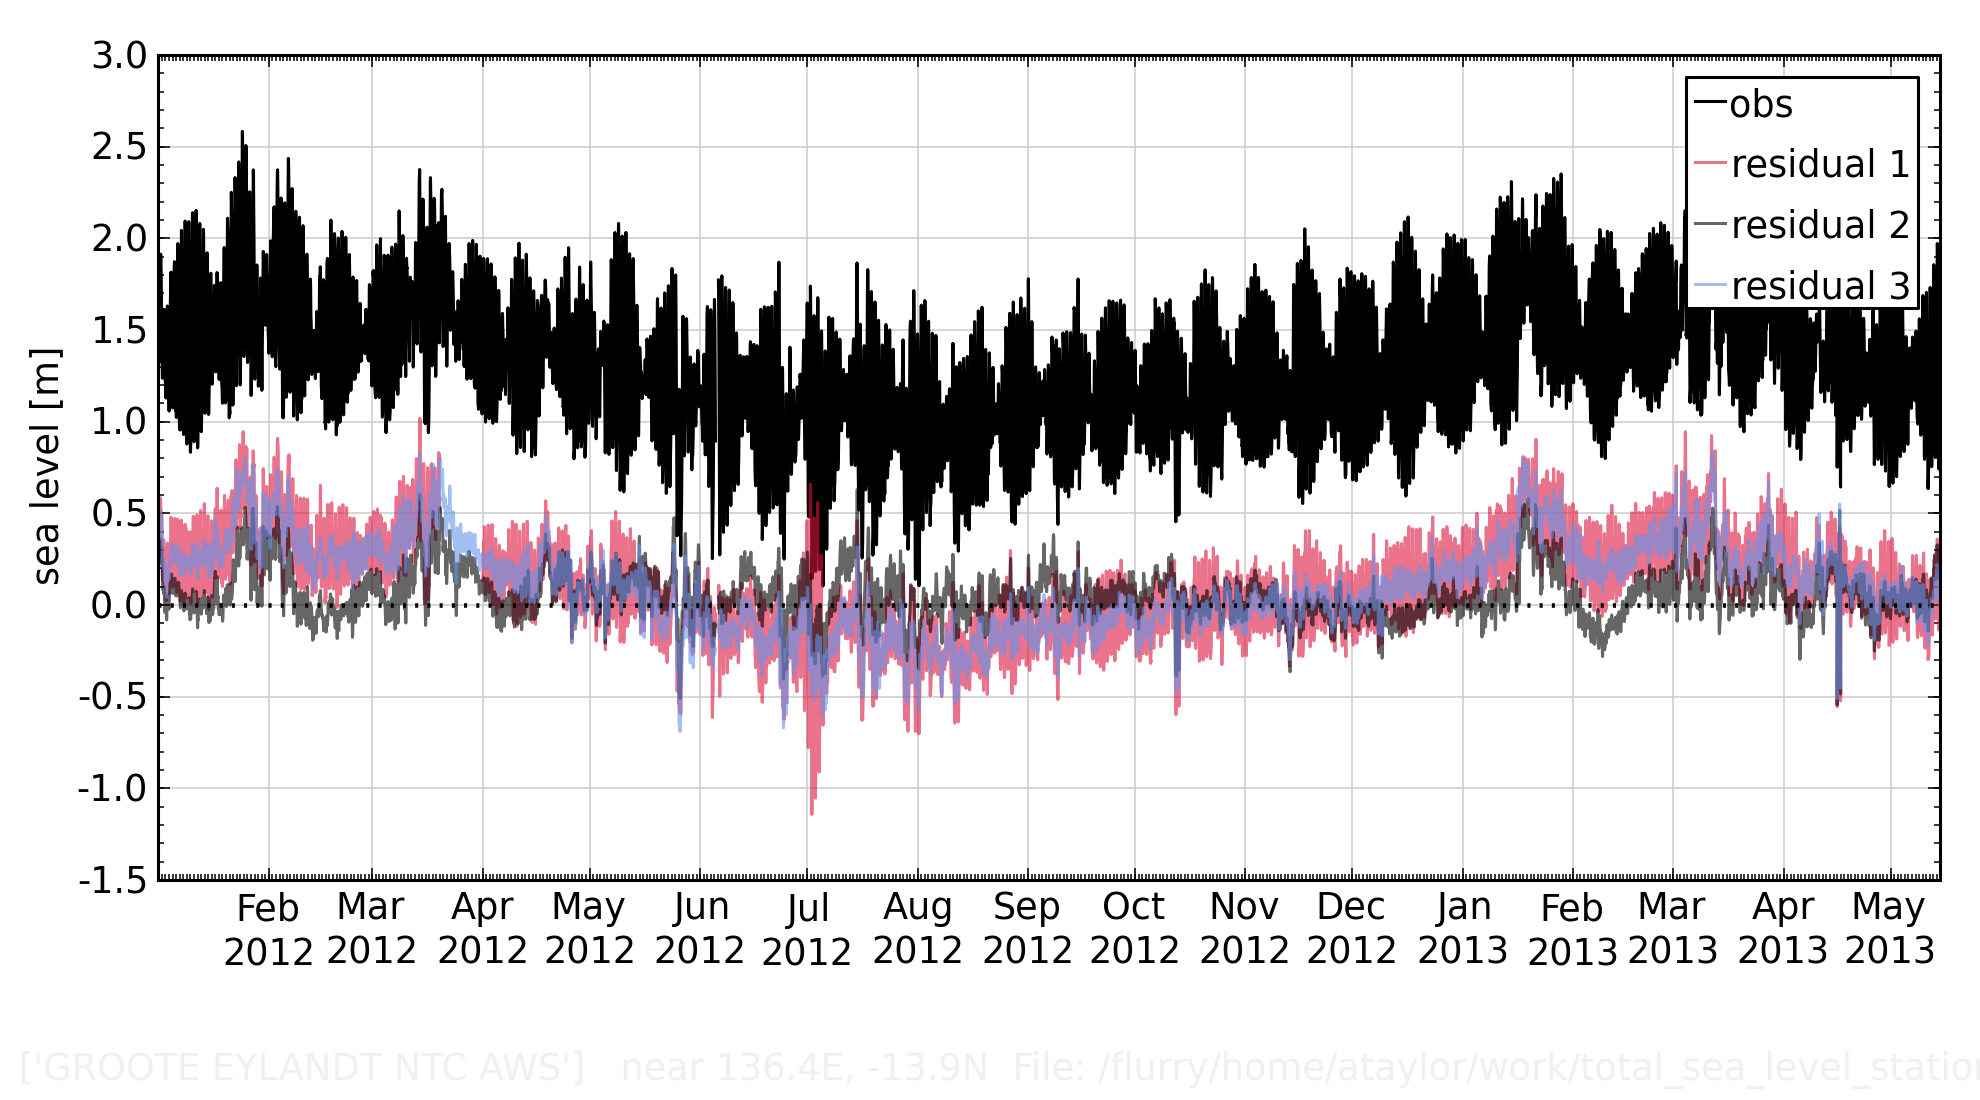
\includegraphics[width=\figwidthFull]{figures/plots/diag_plot_014406_detide_compare_20120101.png}
    \caption{Illustration of de-tiding observations by subtraction of tide predictions.  Different `residuals' result from alternative tide predictions: [1] regional gridded tide solution, [2] harmonic prediction and [3] harmonic prediction with significant non-gravitional harmonics removed. }
    \end{center}
\end{figure}
%-------------------------
Altimetry observations are de-tided via subtraction of a tidal signal synthesised from a global model.  There is no unique manner in which to specify the correction, with many options and `flavours' available from standard sources such as RADS \citep[table 3.2]{Scharroo:2011vd}.  The details of how the tidal correction is constructed can have implications for interpretation of the final ocean forecast.   The treatment of long-period tides \citep{Egbert:2003jd} and nongravitational tides \citep{Arbic:2005gv} are highlighted as special points of interest with regard to operational sea level forecasts.\\




In contrast to the situation with filtering, dynamical cause and effect are only relevant to stand-alone tidal forecast products insofar as they impact predictability.  From a users perspective, tide tables simply forecast sea level and ideally account for as much of the observed signal as possible.   By that measure it is proper that the tide tables include all of the reliably periodic signal regardless of cause.   
Thus the treatment of long-period harmonics Sa and Ssa is `philosophical question' \citep{Parker:2007wq} insofar as any reliably periodic signal at these relatively low frequencies can be determined from the observational record.  It is then not surprising that even amongst Australian tide authorities treatment of long-period signals differs enough to warrant special review attention \citep{MHL2156}.

% wavelets etc
For completeness it should be mentioned that other analysis techniques exist in the literature that are less directly relevant to the provision of sea level forecasts.


For instance, specifically tidal applications of wavelet analysis have been described as tools to provide insight into non-stationary tidal processes \citep{Flinchem:2000kp}.



%-----------------%
\subsection{Spatial tide models}
\label{sec:spatialTides}
Satellite altimetry motivated the extension of the empirical analysis methods discussed above to the production of regional and global atlases of ocean tides.  Indeed, tidal analysis formed an important driver and design constraint on the development of satellite altimetry missions.\\
Global tide models are commonly employed as intermediate products for other calculations well beyond the purposes of sea level forecasting per se.  For instance in the quantification of gravity effects, orbit determination, earth rotation and even the definition of coordinate systems \citep{Anonymous:2004tm}.\\



Meaningful tidal atlases existed prior to altimetry, most significantly that due to Schwiderski \citep{Schwiderski:1983ke}, but these necessarily suffered from a lack of validation and constraint in the deep ocean.\\
The basic premise of a tidal atlas is to present maps of tidal admittance at discrete frequencies, typically as separate amplitude and phase diagrams.   In line with the discussion in Section \ref{sec:LTI}, the deep ocean is conceived as a LTI system that is by definition stationary.  Each component wave can also be called a partial tide.\\
It is conventional to present atlas tidal predictions as separate maps of amplitude and phase for a single frequency.  These are also called `co-tidal' and `co-range' plots.  This visualisation fits well with the concept of the tidal ocean as a linear sum of standing waves.   The long spatial scale of these component waves and the existence of spatial nodes places special importance upon \emph{amphidromes} or \emph{amphidromic points} - nomenclature introduced by Harris in the late 19th century \cite[pp 119]{Cartwright:2000tt}.  Existence and placement of amphidromic points is an important visual metric employed to assess tidal model results \citep{foreman:2012perscomm}.  Figure \ref{fig:atlas} shows a the typical tidal atlas result with amphidromic systems apparent as radial patterns in the co-phase diagram.


Modern tidal atlases are in close agreement with regard to broad patterns, but characteristically differ at the shallow water margins; the very location of most direct interest to sea level forecasts.  Figure \ref{fig:tpx_cross} illustrates the fact that modern global tide models typically agree within about 0.02m in the deep ocean, but can differ substantially in coastal and shelf regions.  
%---------------------------
\begin{figure}[h]
    \begin{center}
    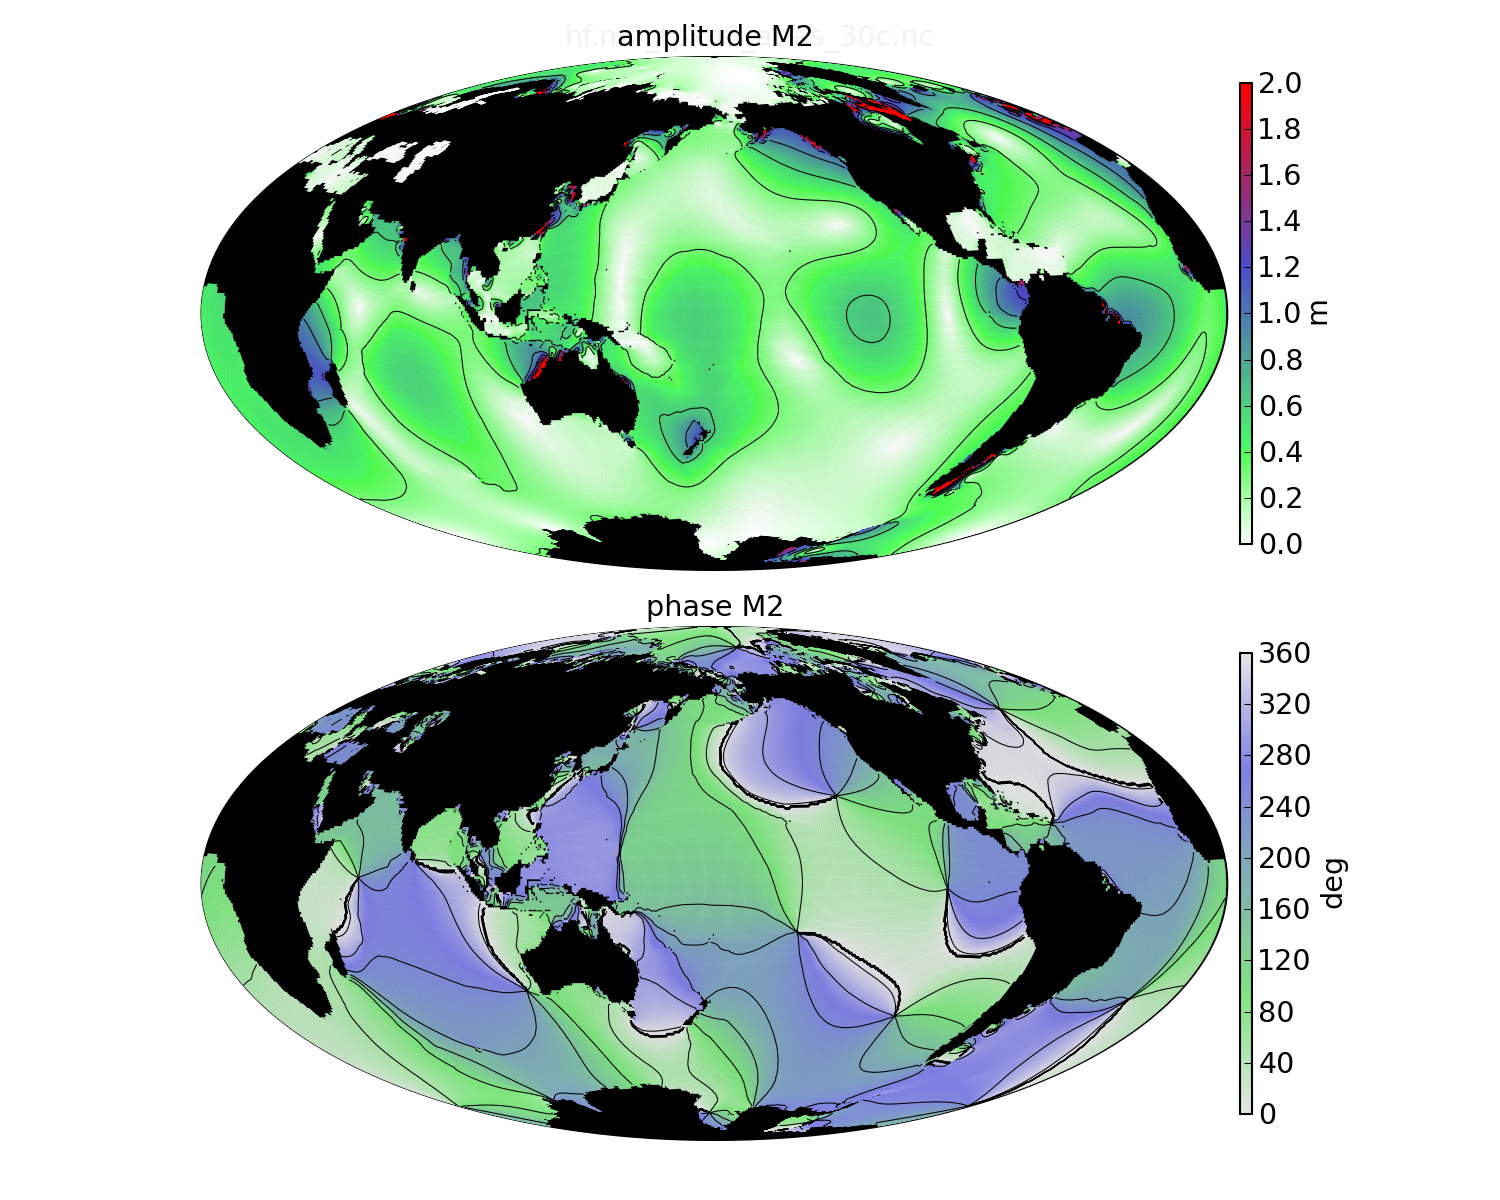
\includegraphics[width=\figwidthBig]{figures/maps/global_m2_tpx08.png}
    \caption{Example tidal altas showing cophase and corange diagrams for a single tidal component M2.  Data source TPX08 \cite{Egbert:2002ug}  }
    \label{fig:atlas}
    \end{center}
\end{figure}
%---------------------------
\begin{figure}[h]
    \begin{center}
    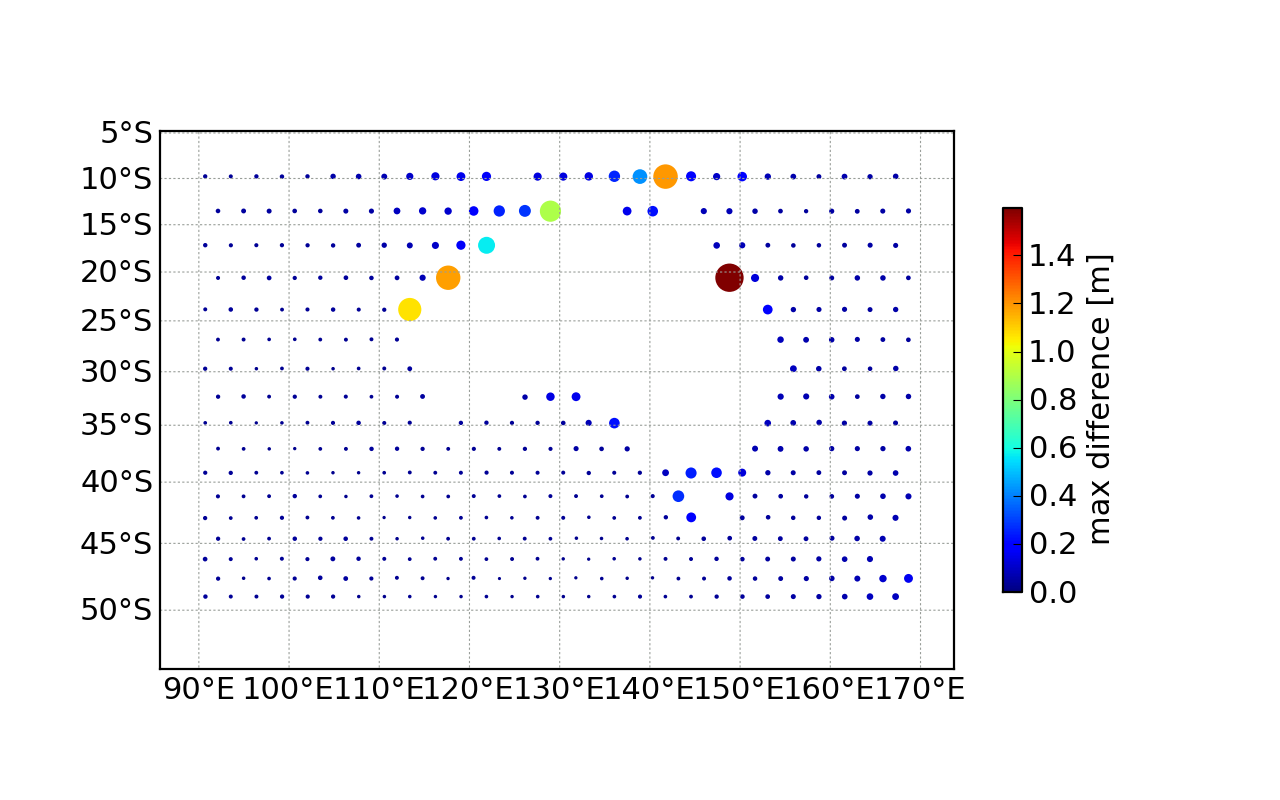
\includegraphics[width=\figwidthBig]{figures/maps/map_tide_differences_tpx_xovers.png}
    \caption{Maximum difference between tidal timeseries for 2012 at topex cross-overs near Australia.  The different solutions agree very closely in deep water, whilst the significance of shallow water effects are apparent.  Models included: CSR04\citep{Eanes:1996tr}, FES04\citep{Lyard:2006ir}, DTU10\citep{IMPROVEMENTOFGLOBA:2010tu}, GOT47, GOT48\citep{Schrama:1994vr}\citep{Ray:1999vm} }
     \label{fig:tpx_cross}
\end{center}
\end{figure}
%---------------------------

The LTI concept embodied in tidal atlases is well suited to representing deep water tides.   Amplitudes of each partial tide are no larger than about 0.02 cm for the majority of the global ocean, compared to depths of around 4km.
Given the underlying LTI framework, the tidal literature has naturally focused on stationary frequency-space metrics.  Intercomparison of mode1s and assessment against observations is almost always performed at a small set of dominant tidal frequencies - commonly only M2, K1, O1 and S2.


Tidal atlases are in essence no different from one-dimensional tide predictions.   Preceding discussions regarding the varied formalisms [Section \ref{sec:formalisms}] apply equally to regional atlases as to insitu timeseries.  Similarly to insitu tidal products, special attention is warranted regarding the treatment of signals associated with non-gravitational effects and the possible differences between a forecast model and an correction/filter.



Whilst some authors have presented the existence of repeat-orbit altimetry observations as effectively being `thousands of tide gauges', reduction of these observations via tidal analysis requires many special considerations.  For instance, infrequent but regular observation of any one surface coordinate places special importance on aliasing effects.



Despite the general equivalence, a point of practical difference is the treatment of the non-linear effects significant in shallow water.
In contrast to the apparent convergence of surface tide models in the open ocean, shelf and coastal regions are problematic.   In shallow waters wavelengths shorten and nonlinear interactions between partial tides can become very prominent.  \\
A strength of conventional 1-dimension analyses of coastal tide gauges has been the incorporation of shallow water compound tides.  It is not atypical in Australian locations to include dozens of nonlinear frequencies in a harmonic analyses.   Nonlinear signals observed at a tide gauge are often due to complex very localised dynamics, and the spatial projection beyond the observation point is non-trivial.  Understandably, global tidal atlases have generally focussed attention on the linear deep water signal and have poorly represented or ignored coastal nonlinearties.  The nonlinear M4 signal (associated with self-interaction of M2 waves) is perhaps the only such partial tide to be included in many modern atlases and is observable with altimetry \cite{Ray:2010jm}.


As a forecast product, tidal atlases have nothing like the broad economic integration of conventional coastal tide tables.  The Australian Bureau of Meteorology does not promulgate official tide predictions away from insitu observation locations. 
For the contemporary operation setting, tidal atlases are primarily relevant as an intermediate product to enable satellite observations.



Coordinated development of improved tidal atlases with specific performance requirements formed a significant component of altimetry missions in the 1990s.
\begin{quotation}
This international effort quickly split into two main approaches: the so-called empirical approach based on the direct analysis of the altimetry sea level time series \dots{}, and a modelling approach based on hydrodynamic and assimilation models. Later on, the interaction between the two approaches (i.e. data assimilation based on altimetry analysis on one hand, and hydrodynamic/assimilation modelling on the other hand) was a key factor for the overall success in improving tidal prediction accuracy and reaching the T/P requirements \cite[pp394]{Lefevre:2011dg}.
\end{quotation}


%%-----------------%
%\subsection{Global tide solutions and data assimilation}

TBC!! 


No global tidal atlas can be purely empirical - the spatial and temporal coverage of observations is too sparse.\\
Schwiderski's pre-altimetry solutions relied heavily on global compilations of harmonic constants for mainly coastal tide gauges, from which spatial maps were created via a `hydrodynamic interpolation' method that would in hindsight be considered an application of data assimilation \cite[pp822]{Egbert:1994wz}.\\
Now with around 20 years of altimetry data, all the highly evolved global tidal models or \emph{tidal solutions} in use all employ data assimilation in some manner.  That is, they make some combined use of dynamic models and observational data.  This includes a reliance on supporting geophysical models and corrections implied by the use of altimetry observations.\\



The dynamics relevant to tidal sea level are conventional written as the Laplace Tidal Equations (LTE) - for instance \cite[9.8]{gill1982atmosphere} and \cite{Hendershott:1981ub}.   
Via a series of assumptions, the LTE are a set of depth integrated shallow water equations in a rotating thin shell.  Advection is neglected altogether.\\
The LTE evolve a simple 3 dimensional ocean state consisting of horizontal mass transport and sea level perturbation. In time domain, the LTE can be written following the notation and discussion of \cite[pp185]{Egbert:2002ug}:
%----------------------
% LTE in time-domain
\begin{align}
    \label{E:LTE_momtm}
    \frac{\delta \mathbf{U} }{ \delta t} + f\vec{k} \times \mathbf{U} + gH\nabla \eta  + \mathbf{F} &= \mathbf{f_0} + gH \nabla \eta_{SAL} \\
    \label{E:LTE_cont}
    \frac{\delta \mathbf{\eta} }{\delta t} &= -\nabla.\mathbf{U} 
\end{align}
%----------------------
Where $\mathbf{U}$ is the depth integrated horizontal transport, $\eta$ is the sea level signal, $H \gg \eta$ is mean water column depth, $f=2\Omega\sin\theta$ is the Coriolis parameter and $g$ vertical gravitation.\\
The forcing terms on the right hand side of the momentum equation \label{E:LTE_momtm} require explanation.  
$\mathbf{f_0}$ denotes the astronomical body forcing taking into account earth tide effects, $\mathbf{f_0} = gH\nabla\eta_{eq}$ following Equation \ref{eq:VT}.  
An approximation for SAL is here written as a separate forcing term to reflect the suitability of using values pre-computed from existing global tide models.   
Alternatively $\eta_{SAL}$ can be put on the left hand side of the equation as a scaled version of $\eta$ - as is the case in \MOM{}.   
This scalar approximation is relatively inaccurate as discussed in section \ref{sec:basic_potential}.\\
The frictional dissipation term $F$ is a particular source of complexity, especially with regard to parameterisation and linearisation.\\

Compared to the dynamics represented within an \OGCM{}, these tidal hydrodynamics simulate a more `aggregated' psuedofluid in that the processes contained within parameterisations are have a higher degree of complexity - as per the schematic in Figure \ref{fig:models} \\
\begin{quotation}
Forward global tide models are an ideal testing ground for the hydrodynamical cores of numerical ocean general circulation models, and for ideas about drag and dissipation. In contrast to data-constrained models, forward models cannot achieve accurate tidal elevations unless substantial parameterised drag is included in the abyss. Forward models thus point clearly to drag in the open ocean as a central control on tidal flow.\citep{Arbic:2004wz}
\end{quotation} 


Linearisation is important in the tidal context to facilitate transformation of the LTE into the frequency domain.   Given the tidal LTI framework, the ultimate solution of a tidal model is the evaluation of static admittances or constants.   One approach towards this end would be to integrate the LTE in the time-domain and subsequently reduce the output to a series of harmonic constants via conventional analysis.   The celerity of barotropic waves in the deep ocean is relatively fast and thus requires short time-steps.   Assuming linearity and the existence of a convergent solution in frequency-space, the LTE can be solved directly in spectral form with greater computational efficiency.   The efficiencies are especially important upon the application of data-assimilation methods that involve both a backward and forward iteration of the dynamics \cite[pp184]{Egbert:2002ug}.


Again following the notation of \cite[pp186]{Egbert:2002ug}, the LTE at a single tidal frequency $\omega$ can be written:
%----------------------
% LTE in freq-domain
\begin{align}
\label{E:LTE_momtm_w}
\mathbf{\Omega} \mathbf{U} + gH\nabla \eta &= f_u \\
\label{E:LTE_cont_w}
\nabla.\mathbf{U} + i\omega\eta &= f_\eta\\
\mbox{where   } \Omega             &=
\left[ \begin{array}{cc} 
      i\omega + \kappa & f \\ 
       -f              & i\omega + \kappa  
                        \end{array} \right]   \nonumber
\end{align}
%----------------------
Where $\kappa$ is a linearised approximation for the dissipative stress.   Frequency-space forcing terms $f_u, f_\eta$ are written in both equations for generality with regard to data assimilation (inversion).  This frequency-space approach is common to other data assimilative tidal models such as FES \cite[pp395]{Lyard:2006ir}.\\
Nonlinear terms can be incorporated but complicate the formulation of any inversion.


Whilst numerically solving the LTE is quite tractable and comparatively simple, significant uncertainties prevent a direct `free' or `forward' model from producing accurate forecasts.  Hence the importance of data assimilation or generalised inversion methods.  Solving the LTE is complicated by spare observations and ``$\dots$ the need for accurate open boundary conditions and bottom topography, the need for approximate parameterisations of dissipation in the tidal equations, solid earth effects, and the effects of ocean stratification on the barotropic tides, which may be difficult to account for without full 3D modelling of baroclinic tidal currents''\citep[183]{Egbert:2002ug}.

A comparative description of data assimilation methods in the context of tide models is laid out by Egbert and Bennet \cite{Egbert:1996vr}.



Summaries that categorise the many global tide models on the basis of design choices, parameterisations and data assimilation methods are given in \cite{Ardalan:2008gs} and \cite{Matsumoto:2000tg}. \\

%   ??  Application of the LTE is not restricted to the barotropic surface tide.   The formulation can be extended to represent stationary internal tidal modes via use of equivalent-depths .\\
% Energy cascades.??\\

The barotropic hydrodynamics used in global tide models has proven to be an appropriate level of aggregation when the aim is to map tidal patterns of surface elevation.  The LTE provide a tractable means of doing so given the incomplete spatial and temporal coverage of observations.

But consideration of tidal dynamics naturally raises the topic of \emph{internal tides} and the separability of stationary barotropic tides from other ocean dynamics.
\begin{quotation}
Barotropic tides generate internal tides, and internal tides in turn feed back onto the barotropic tides. Inferences from altimetry-constrained barotropic tide models show that about one-third of global tidal energy dissipation occurs in regions of rough topography, where internal tides are generated \dots{}. Internal tide generation thus acts as a damping mechanism for the barotropic tides.\citep[pp22]{Arbic:hy}
\end{quotation}
Depth integrated barotropic LTE relegate the effect of internal mechanisms on surface elevation to parameterisations.  Dissipative stress $F$ in \label{E:LTE_momtm} stands for all losses of energy from the barotropic pseudofluid.  Given the reality of ocean stratification, these losses notably include conversion form the barotropic to higher baroclinic modes \cite[pp121] {gill1982atmosphere}.


For the present topic of sea level forecasting, internal modes are ostensibly of interest insofar as they impact the prediction of surface elevation.  Internal waves at tidal frequencies do have an observable surface signature albeit relatively small \cite{Ray:2011tj}.

More importantly for forecasting is the effect of the internal ocean state on the prediction of barotropic surface elevation.  A-periodic variation of the internal density structure of the ocean is of particular relevance as   conventional tidal analysis relies upon periodicity for predictability.     The tidal view of the ocean as a LTI system driven by the \ATGP{} is very useful, but with the caveat that ``the ocean is a physically complex and noisy filter.  In consequence, tidal harmonics are not strictly constant \citep[197]{Ray:2010jm}''.


Whilst stratification and internal mechanisms are very coarsely parameterised in dedicated tidal models, the internal structure of the ocean is a primary focus of \OGCM{}s.   The following section addresses the intersection of \OGCM{}s and tidal forcing with regard to sea level forecasts.


%-----------------%
\subsection{No singular ocean tide requirement in operations}

TBC .... 
whereas tidal manuals exist such as \citep{PCTMSL-sp9}, \citep{IOC:2005tj}, \citep{Level:2011wu}and \citep{Parker:2007wq} the operational details of practices are not generally published. 



A range of auxillary and derived from conventional tidal methods
- reference planes like HAT
- 



This lack of clarity motivates proposal in Chapter \ref{chp:tideFlavours}



detiding filter for non-tidal models taken up in the next section ....
\section{Exploiting existing predictability}
\label{sec:exploitingPredictability}
%--------------------
\subsection{Unresolved processes and overlap}
All sea level forecasting systems are realised via design choices regarding what processes are in scope and the manner in which they are represented.
In the above sections, two operational approaches were contrasted; tide prediction and scale-limited hydrodynamic ocean circulation simulation.
To a first approximation these forecast types are conceptually complimentary; one being tidal and the other non-tidal, one in which the ocean is characterised by a time-invariant admittance and other by the evolution of a turbulent fluid. 
Each approach necessarily must account for the impact of unresolved processes on the target representation.


There are reasons to look critically at the nominal separation of these tidal and non-tidal forecast approaches.
Most simply, the fact that more than one conceptualisation of what comprises tidal sea level is in use operationally requires, at a minimum, semantic care to avoid misunderstanding.
More fundamentally, the boundary between resolved and unresolved will be redefined as simulation systems are updated and improved.  Hydrodynamic simulation in particular is set to continue in a direction of ever-higher fidelity and concreteness.

The motivation to explicitly represent tides in \OGCM{}s provides a clear case where the separation between tidal and nontidal would require revision.   
But some representation overlap of this nature is already present and is taken up in chapter \ref{chp:tideFlavours}.


Increasing simulation fidelity, moving processes from unresolved to resolved, is of itself not necessarily beneficial for forecast value.
Forecast value is ultimately found in the predictability of an actionable quantity.  


Consider by analogy the case of spectral wind wave forecasting. 
Wave forecasting is like tide prediction essentially a stand-alone bespoke numerical forecasting method.   Operational wave forecasts represent the sea level variability within certain time and length scale limits as a time-evolving spatial map of spectra. Bulk spectral properties such as significant wave height are usefully predictable out to several days and are in wide use for navigation and other applications.   However, these predictable spectral properties are not directly observable sea level per se.   Increasing simulation concreteness to the degree of forecasting waves in a phase-resolving framework (as in the littoral forecasts described by \citep{10.1080/1755876x.2019.1685834}) is not yet tractable for large domains over long forecasts; and may not ultimately prove to offer any more actionable value for many applications than the existing spectral approach does.



Conventional tidal analysis has established a unique manner in which to extract a specific type of predictability from historical point observations.
The projection (fitting) process is designed to sift out patterns of variability that have been sufficiently coherent with the temporal variability of the \ATGP{}; without any knowledge of the environment beyond the forecast location.

But extension of tidal analysis beyond in situ observation points necessarily intersects with hydrodynamics; which in turn includes drawing a boundary between resolved and parameterised processes.  

A key tool for handling unresolved processes in both operational mesoscale ocean forecasting and global tide spatial solutions is data assimilation; optimally \textit{fitting the data and the dynamics ``well enough''} \citep{Egbert:1994wz}. 
But the target of ``well-enough'' is not isomorphic between the two forecasting approaches.
Whereas global tide solutions seek an optimal time-unvarying balance between simplified shallow water dynamics and observations in tidal frequency space, the mesoscale forecast requires a best-guess initial condition for the ocean circulation state.  
Despite the difference in detail, both are similar in that they draw trade-offs to provide an overall spatially consistent optimal representation.   Neither are optimised for a single location or user.

Operational sea level forecasting in contrast, could be considered as an isolated and targeted activity for which additional assimilation or data-driven approaches could be applied in order to extract the most relevant predictability. 

%--------------------
\subsection{Sea level forecast development}
\citet{10.3389/fmars.2019.00437} review and summarise the current state and direction of coastal sea level monitoring and prediction.   These authors emphasise the complex mix of processes and ``our limited capacity to predict [sea level] at the coast on relevant spatial and temporal scale''.
Their motivation towards \emph{comprehensive} systems is essentially the same as what has here been termed seamless services. 
They name three directions for development:
\begin{quote}
(i) the use of realistic numerical models to resolve the processes that govern the ocean dynamics; (ii) the use of observations, which combined with statistical techniques are used to identify space and time patterns and extrapolate them into the future , and (iii) the hybrid approach, which combines the first two in a wide variety of ways.
\end{quote} 

Arguably, the current state of the first of these directions is represented at the mesoscale by \BL{}.   The second direction starts with the established practices of conventional tidal analysis.

One instance of the third hybrid direction is explored in chapter \ref{chp:aggregate} with the direct combination of existing operational systems.
Managing any such hybrid forecasting system across future evolution of the operational suite will involve more than just the transitions from higher to lower fidelity with forecast range.  Rather, more qualitative transitions will be involved between tide-resolving and tide-excluding simulations against a time-scale-spanning reference tide prediction.  Arguably this trajectory doesn't fit so neatly in the chain-of-scales metaphor used to promote the seamless ideal \citep{10.1175/bams-87-9-1195}.


As new dynamic ocean forecasting systems progress as candidates for inclusion in the operational suite, there will be a continual need to characterise and evaluate the representation of sea level provided.  Given the broad mixture of time and length scales expressed in coastal sea level, no model evaluation can hope to be based on a single metric.    The value of focusing some evaluation directly on coastal propagation is taken up in chapter \ref{chp:waveguide}.



But from the operational perspective there is more to sea level forecasting development than the quantification of the skill of the forecasts themselves.
One such aspect is the unique established role of conventional tide prediction.   The use of products such as tide tables is not only deeply embedded into day-to-day activities of coastal communities, but is to varying degrees built into legislation (eg \citep{AusNavAct2012}).   Any improvements to sea level forecasting will be carried out against a background of the concept of an ``official'' tide prediction and associated spatial references like chart datum and highest astronomical tide (HAT).    
This general topic is taken up in chapter \ref{chp:tideFlavours}.


The primary role of in situ observations presents several mundane but fundamental challenges for operational forecasting.
Managing basic metadata and quality control for near-real-time sea level observations is a non-trivial task, which is rendered all the more difficult by the heterogeneity operators and instruments in the Australian context.    Tide gauge instruments are installed and operated by a wide variety of private and public organisations, and given the huge spatial extent of the Australian coast any available observation source is potentially valuable. 
This situation can be contrasted against the significant progress in collating global datasets of research quality archives, or even the efforts to expand monitoring beyond these traditional instruments as discussed in \citet{10.3389/fmars.2019.00348}.



Finally, working towards seamless sea level forecasts in an operational setting will require conceptual clarity about the types of predictability offered by an evolving but imperfect suite of operational systems. 
This collection of operational capabilities will inevitably evolve, and almost certainly never be cleanly complimentary; but the operational requirement for the best available sea level forecast is immediate and ongoing. 
Thus there is value is establishing benchmarks for the forecast value available immediately from existing systems and for preparing the way for the introduction of ever more dynamically inclusive modelling, in the development direction that \citet{Petersen:2012tr} names as increasing the ``concreteness'' of prognostic simulations.








		
\chapter{Methods}\label{c:methods}

%=========================================================================

\begin{synopsis}
This chapter documents the datasets, data analysis procedures and computation procedures common to all results presented in the thesis.
\end{synopsis}

\section{Data}\label{s:data}

%===========================

\subsection{Overview}
Text here.


		\chapter{Conclusion}
\label{chp:conclusions}
This desktop study was motivated by the consideration of sea level from within the Australian Bureau of Meteorology, and certain conceptual problems identified behind operational developments.
Exploration of the intersection of conventional tide prediction and operational mesoscale ocean forecasts within the agency has highlighted nuanced issues of representation, system compatibility and user expectation that are relevant to the strategic direction towards ``seamless'' services.
As such, all evaluations treated here have intentionally not pursued higher fidelity coastal simulations, but instead directed attention to some less-studied aspects of evaluating and exploiting predictability with established operational systems.   

As a thesis with publication, much of the body of this document has been published as, or is in preparation for peer-reviewed academic papers.
%------------------------
\section{Findings summary}
In answer to the research questions posed in chapter \ref{chp:introduction},  the findings of this thesis are summarised as follows:\\

Firstly, it was demonstrated that incompatible definitions of ocean ``tide'' are in parallel operational use.
Whereas downscaling for coastal sea level forecasts is clearly a productive approach, mesoscale ocean forecasts can immediately and directly provide significant but qualified forecast value for coastal sea level.
The fact that nominally tidal signals are present in mesoscale non-tidal ocean simulations means that care is required to avoid misinterpretation.

An aggregation approach that combines existing heterogeneous data but accounts for double-counting provides an important skill benchmark for future sea level forecast system development.
The point-based bias correction characteristics from these aggregated forecasts indicate that coastally contiguous extensions to model aggregation may be feasible.


In the operational context of combining and upgrading forecast models, it was shown that the coastal propagation characteristics of candidate forecast systems can be usefully evaluated and compared in a grid-independent waveguide projection.
Such a coastal waveguide projection also offers a means to direct forecaster attention to signals of special relevance along the Australian mainland coast.

Finally, it was argued that conventional harmonic tide predictions are not redundant, despite the ongoing advances in hydrodynamic simulation,  but that operational tide services require appropriate product differentiation to compliment modern applications and facilitate future refinement.
     % <<-- external file

%------------------------
\section{Heterogeneous simulations and seamless services}
The original coinage of "seamless" prediction in the context of climate projections has evolved to now encompass the more general goal of prediction across time and length scales \citep{10.1127/metz/2020/1048}.
Indeed the development of more seamless services is a strategic goal of the Australian Bureau of Meteorology \cite{BOM2020}.
\cite{10.1175/bams-89-4-459} illustrated the concept with a schematic chain of scales reaching from the small and fast out to the large and slow.
The present focus on sea level forecasting allows for a twist on the chain image to highlight the unusual place in which the LTI tidal admittance approach can be located relative to the geophysical fluid suite of simulations.
Figure \ref{fig:forecastScalesChain} schematically shows that tide prediction in general can provide very long horizon prognoses of short time scale fluctuations in sea level; of course subject to many caveats.
%------------------------------
\begin{figure}[h]\centering
        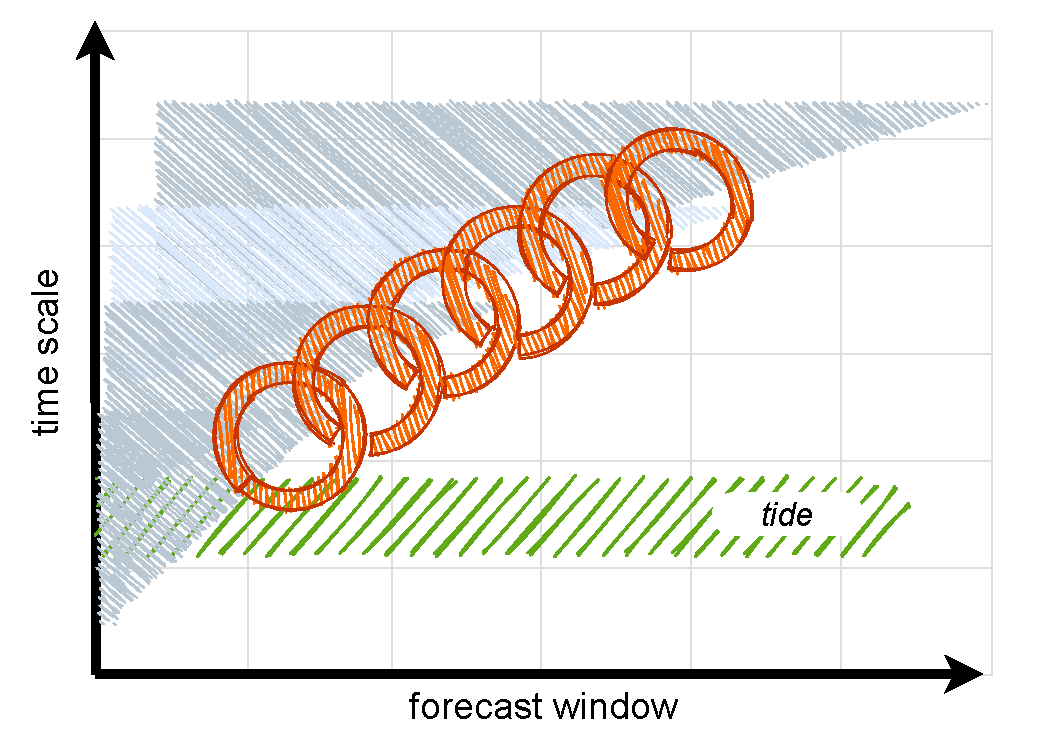
\includegraphics[width=\figwidthFull]{figures/diagrams/scales_with_chain.pdf} 
        \caption{Tide prediction can sit awkwardly with the seamless chain-of-scales analogy and highlights an ongoing role for system heterogeneity; following Figure \ref{fig:forecastScalesAll} and \citep{10.1175/bams-89-4-459}}
        \label{fig:forecastScalesChain}
\end{figure}
%------------------------------
The intention behind this imagery is to emphasise that multi-scale prediction need not be shoe-horned into the tidy cascade of a single consistent earth system simulation framework.
Although a consistent framework and a single simulation code-base is very attractive on multiple fronts  \footnote{\url{https://research.csiro.au/access/what/}}, consideration of the status of sea level and tide prediction provides at least one case in which some sort of exception is sure to be required based on the unique value offered by particular mechanisms and legacy products.  

Operational forecasting today, when viewed holistically, is based on a suite of systems that are not cleanly compatible.
The prognostic potential of Australian Bureau of Meteorology has arguably not been fully realised to some degree as a result of system heterogeneity.  Consider how the forecast information published variously as maps of non-tidal sea level anomaly, storm surge warnings and tide-table products cannot self-evidently be synthesized and directly interpreted in relation to observable sea level.
And whilst progress towards ever more concrete and consistent earth simulations will continue apace, there is sure to be an ongoing operational requirement to handle inhomogeneity and system transitions in manner that actually provides useful forecast value. And in line with the final recommendation of \cite{10.1175/bams-89-4-459}, realising that value will require ``\textit{closer and wider cooperation between the scientific community, stakeholders, policy- and decision-makers to ensure that sea level products are accessible and are used correctly and appropriately...}''. 

%------------------------
\section{Next steps}
The will be ongoing opportunities to improve sea level forecast services as the operational suite of simulation systems improve, but any innovation will necessarily be interpreted by users against the background of conventional tide predictions.

Whilst this body of work intentionally restricted focus to the Australian setting, some of the higher level  characterisations will be translatable to other shores.  Especially the basic conceptual overlap between aspects of conventional tide prediction and hydrodynamic simulation.
The federated jurisdiction combined with the vast expanse of the Australian coast tips the balance of operational challenges towards delivering a more universal, as opposed to highly targeted, approach to forecasting.   As a jurisdictional contrast is available in the case of South Korea, where a dense network of weather and marine observations are maintained under the same auspices as the forecasting agency (eg   
\citep{10.1007/s10236-015-0820-3}).
The vast Australian coast also raises the significance of large scale coastal propagation, and moreover highlights the problem of observation sparsity.


There remains a primary role for \underline{tide gauge observations} to underpin sea level forecasting across the board.
Expansion of the observation capabilities to new platforms, be it video \citep{10.1175/jtech-d-18-0203.1} or wide swath altimetry, will not side-step the ongoing role for tide gauges.
\cite{Keysers:we} emphasised the need for not only a denser network of observations around the Australian coast, but a national repository and ongoing curation of sea level observations and survey connections to support the needs of precision positioning.   
That call is effectively mirrored for forecasting applications in the recommendations of \cite{10.1175/bams-89-4-459}.
As yet, there is no such Australian coordination; at least not in the sense of seamlessly serving real-time and survey applications.
There is an obvious opportunity to better align the capabilities of the conventional tide service, operational forecasting and spatial survey to maintain a foundational public resource.  Whilst small steps have been taken in that direction by the Intergovernmental Committee on Surveying and Mapping \footnote{\url{https://www.icsm.gov.au/}}, progress would be a great enabler for improved sea level forecast services.





Finally, consideration of how tides and sea level fit within the operational setting of the Bureau of Meteorology corroborates the need for a concept of forecasting services that juxtaposes the chain-of-scales model; namely the so-called `micro-service' architecture \citep{BCG2020}.
Quite apart from the vision for an all-encompassing multi-scale earth system simulation, the extraction of value from forecasts more generally appears to be on a fast trajectory towards the downstream combination of heterogeneous inputs for bespoke decision support applications.
Ensuring that forecast outputs of all sorts are machine-readable, discoverable and well-characterised will facilitate the development of improved sea level applications both within and external to the operational agency itself.    

%is increasingly relevant to government services and is embodied by programs such as  \url{api.gov.au}) and the International Hydrographic Organisations  navigation-focused exchange specifications (\url{http://s100.iho.int}).




	\end{mainmatter}
	%---------------
	% bibliography
	%---------------
	\addcontentsline{toc}{part}{Bibliography}		
	\bibliography{bib/references}
	%---------------
	% appendices
	%---------------
    \begin{appendix}
		
\chapter{More on tidal formalisms}
\label{appendix:response}

\section{Response}
Godin \citep{Godin:1991vx} describes the response method as `cross spectral analysis'; a LTI model is inverted from comparison of the input and output timeseries.   
Whereas harmonic methods evolved well before the availability of machine computers, the response method relies on computational signal processing with discretely sampled and finite length time series.


A response analysis aims to empirically characterise the LTI as a complex-valued transfer function on the basis of output coherence with the input/s. 
\begin{quotation}
The goal of any response formalism is to accurately predict the ocean tides by an optimum smooth function, realising that the ocean tides are mostly, although not completely, predictable.
\end{quotation}

Note that the outcome of a response analysis is not a single admittance curve, but rather a small number of distinct curves; typically the semi-diurnal, diurnal and long-period tides associated with degree-2 spherical harmonics $(n,m)=(2,2),(2,1),(2,0)$.\\
Smoothness of $Z(\omega)$ within each distinct tidal band is a core principle behind methods for determining admittances.  

\begin{align}
\label{E:response}
g(\Delta t) + \dots &\Rightarrow & \fbox{empirical admittance curves $Z$} &\Rightarrow & \mbox{$\eta(\Delta t)$}  %\nonumber
\end{align}

Once determined, admittance curves map a tidal input timeseries to an output timeseries.

% admittance
\begin{equation}
\label{E:Z}
\eta(t) = \sum_{n=2}^{3}\sum_{m=0}^{n}\sum_{k} H_{nmk} \text{Re} \left[ Z_{nm}(\omega)^*e^{-i(t\theta_{nmk})} \right] 
\end{equation}


The presence of incoherent noise in the observational timeseries means that determining $Z$ is not simply the matter of division in frequency-space.\\



In order to distinguish coherent signal from incoherent noise, Munk and Cartwright introduce the \emph{convolution formalism}. The convolution technique exploited the band-concentration of tidal spectra into semi-diurnal, diurnal and long period species and the associated assumption of \emph{smooth} admittances within each of these bands.  A complex-valued admittance $Z(i\omega)$ is fitted separately to each band-limited species via a convolution operation in time-space. 
Inversion of a smooth admittance function from tidal records can be classed as a discrete-time/continuous-frequency operation \citep{Percival:1998tw}.\\

There is however, no unique manner in which to formulate the problem.  Munk and Cartwright formulated the convolution with a discrete time-kernal of `lag weights' as in equation \ref{E:lags}.   This is equivalent to modelling the smooth admittance in each band as a finite (and periodic in frequency) Fourier series.   Although no physical meaning is attributed to the periodicity of the admittance in frequency, in the context of band-concentrated tidal energy, this allows for a compact convolution kernal consisting of only a very small number of `lags`.   The design of this convolution kernal requires a choice of the number of lags $s$ and lag interval $\Delta T$.  Equivalently, this design sets the period and number of Fourier components used to model the admittance function.  For instance, in an application of this convolution formalism to altimetry data, Smith \citep{Smith:1997ut} choose $\Delta T=2$ days and $s=3$.   Note that what at face value may seem a rather long lag of 2 days relates to the \emph{bandwidth} of the tidal species rather than a timescale of tidal variation.\\
From this perspective, a tidal signal is written as a weighted sum of past (and possibly future) values of the driving input function.  \\ 
Tidal analysis consists of empirically determining the weights $w_{nm}$ via a least-squares minimisation on an observational timeseries.\\
The resultant complex weights $w_{nm}$ form a time-space kernal representation of the admittance $Z(\omega)$ in equation \ref{E:Z}.   In frequency-space, the minimisation problem amounts to fitting the Fourier series to model $Z(\omega)$.\\

\begin{align}
\label{E:lags}
\eta_{tidal}(t) &= \sum_{m=0}^{2}\sum_{s=0}^{S} w_{nm}(s)c_{nm}(t-s\Delta T)\\
              n &= 2   \nonumber
\end{align}

The introduction of response methods in the 1960's was not motivated by a user-driven need to improve tide predictions.  It could rather been seen as a move to review the well-embedded conventions of harmonic analysis in the contemporary language of timeseries analysis and ``make explicit what the harmonic method does anyway''\citep[pp 540]{Munk:1966ts}.  In contrast to the dynamic blindness of conventional harmonic analysis, the response perspective facilitated explicit treatment of drivers other than the \ATGP{}.\\

Nonlinear effects are especially significant in coastal locations.   By definition, such shallow-water tides cannot be represented by a LTI model with only $\eta_{eq}$ as an input.  The response method can incorporate nonlinearity as an additional explicit input.    For instance,  in a 2-stage process, a preliminary linear analysis determines admittances for `equivalent deep water port' which are subsequently used to produce new input timeseries of paired and tripled products \citep[pp 122]{Pugh:1996uz}.\\

\begin{figure}[h]
\begin{center}
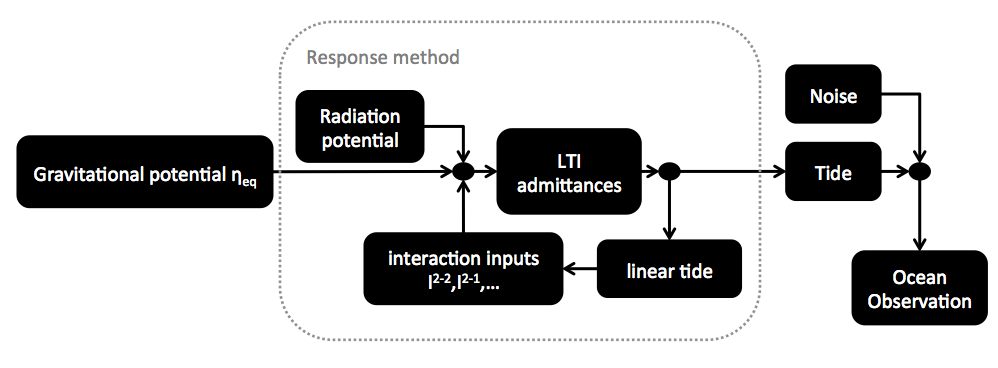
\includegraphics[width=\figwidthBig]{figures/diagrams/response_analysis_flowchart.png}
\caption{Response method tidal schematic.  Nonlinear and non-gravitational inputs are explicitly formed.   Analysis consists of empirically fitting smooth admittance curves.}
\label{fig:response}
\end{center}
\end{figure}

Perhaps even more illustrative of the way in which a response analysis conceptualises tides is the formulation of the `radiational potential'.   This is an additional harmonic forcing series formulated to more explicitly account for the influence of atmospheric tides and other periodic solar effects on ocean observations.	  So-named due to the abstract connection with diurnal solar radiative fluxes, the radiational potential is concept is a little ad hoc in comparison to developments of the \ATGP{}.  The radiational input provided a more satisfactory formulation of observed harmonic ocean signals, S1 and S2, with amplitudes disproportionate to terms in the \ATGP{}.\\
From a sea level forecasting perspective, the response approach could be said to have modernised the formulation and increased the concreteness of the underlying physics, but in doing so hasn't ultimately provide anything more robust and simple for routine use in operational centres.


%\subsection{Variants}
Fitting a Fourier series vi the convolution formalism to find each smooth admittance is not the only viable implementation of the response concept.  For instance a Green's function formulation is described by \citet{Webb:1974ke} and polynomial models are evaluated by \citet{Desai:1995je}. More influential though is the orthotide approach to fitting Fourier series admittances, discussed below.




\section{Orthotide}% orthotide
A possible weakness of the original convolution formalism in equation \ref{E:lags} relates to the non-orthoganality of the harmonically decomposed $c_{nm}(t)$.  That is, unlike a Fourier series, inner products between component sinusoids comprising the tidal input are not necessarily zero.   Thus the resultant weights $w_{nm}(s)$ are dependant on details of the particular analysis, such as the number of other components included.  The weights cannot be assigned any independent meaning and are not amenable to communication.  In recognising this, Groves and Reynolds \citep {Groves:1975ky} introduced the \underline{orthotide formalism}.\\
Orthotides are orthogalised transformations of the harmonically decomposed tidal input timeseries.

\begin{align}
c_{nm}(t) =  &\sum_{k} H_{nmk} e^{-i(\omega_{nmk} + \beta_{nml})}  \Rightarrow \sum_{l}^L \overline{\zeta}_{nml}(t)     \nonumber \\
             &\mbox{where} \langle \overline{\zeta}_p \overline{\zeta}_q \rangle  = \delta_{pq}  \mbox{over $-\infty < t < \infty$}             \nonumber
\end{align}

A tidal timeseries is then represented as a linear sum of these orthotide functions with `orthoweights'. In essence this is no different to Munk and Cartwrights convolution, but is an improved time-space formulation of equation \label{E:Z}.  The resulting orthoweights have the attractive property of not being dependant on the number of components involved in any particular analysis, and subsequently could be said to share some of the characteristics of conventional tidal constants.
\begin{equation}
\label{E:orthosum}
\eta_{tide}(t) = \sum_{n=2}^3 \sum_{m=0}^n \sum_{l}^L \overline{\zeta}_{nml}(t)
\end{equation}

Regardless of the formulation of time-space convolution, the determination of weights is equivalent to fitting smooth admittance curves - which is the ultimate goal of the response method.  The fitting process is a minimisation problem with degrees of freedom equal to the number of free parameters to be determined.    The length of timeseries and signal to noise ratio are balanced against the assumption of smoothness in $Z$.
\begin{quotation}   
The use of orthotides may provide some benefits to the empirical determination of ocean tide models from a short duration of observations, but is otherwise unnecessary. \dots  polynomial and orthotide, and therefore convolution, approaches to modelling the smooth admittance function provided similar results as long as they are defined by an identical number of parameters.\citep{Desai:2006wo}
\end{quotation}

	\end{appendix}
\end{document}
